%\documentclass[options]{class}
\documentclass[12pt, twoside]{report}

%Para listado de programas
\usepackage{listings}
\usepackage{color}

\definecolor{mygreen}{rgb}{0,0.5,0}
\definecolor{mygray}{rgb}{0.7,0.7,0.7}
\definecolor{mymauve}{rgb}{0.58,0,0.82}

\lstset{ %
	backgroundcolor=\color{mygray},   % choose the background color; you must add \usepackage{color} or \usepackage{xcolor}
	basicstyle=\footnotesize\ttfamily,        % the size of the fonts that are used for the code
	breaklines=true,            % Zeilen werden Umgebrochen
	keywordstyle=\color{red},
	commentstyle=\itshape\color{mygreen},    % comment style
	numbers=left,                    % where to put the line-numbers; possible values are (none, left, right)
	numbersep=5pt                   % how far the line-numbers are from the code
}

%Paquete de Idioma
\usepackage[spanish]{babel}

%Codificación Alfabeto
\usepackage[utf8]{inputenc}

%Codificación de Fuente
\usepackage[T1]{fontenc}

%Índice
\usepackage{makeidx}

%Gráficos
\usepackage{graphicx}
\usepackage{float} 
%\usepackage{xcolor} 

%Matemática
\usepackage{amsmath}
\usepackage{amsfonts}
\usepackage{amssymb}
\usepackage{amstext} 

%Estilo de Página Numeración superior
%\pagestyle{headings}

%un estilo propio
\usepackage{fancyhdr}
\setlength{\headheight}{15pt}

\pagestyle{fancy}
\renewcommand{\chaptermark}[1]{ \markboth{\chaptername\ \thechapter: #1}{} }
\renewcommand{\sectionmark}[1]{ \markright{ Sección \thesection. #1}{} }

\fancyhf{}
\fancyhead[LE,RO]{\thepage}
\fancyhead[RE]{\textit{ \nouppercase{\leftmark}} }
\fancyhead[LO]{\textit{ \nouppercase{\rightmark}} }
\fancyfoot[CE]{\textit{\textcopyright 2015 Laboratorio de Sistemas Embebidos\\
	                    UPAEP} }
\fancyfoot[CO]{\textit{LSE001-2015 \\
		Elaboró: Dr. Casimiro Gómez González} }	            
\fancypagestyle{plain}{ %
	\fancyhf{} % remove everything
	\renewcommand{\headrulewidth}{0pt} % remove lines as well
	\renewcommand{\footrulewidth}{0pt}
}

%Hiperlinks \href{url}{text}
\usepackage[pdftex]{hyperref}

\usepackage{cite} % para contraer referencias

%Titulo
\title{LSE001-2015: Conceptos Básicos de Python}
\author{Dr. Casimiro Gómez González\\
	Facultad de Electrónica, UPAEP\\
               correo: casimiro.gomez@upaep.mx\\
               Tel: 222 229 9428}
\date{Primavera 2015}

\begin{document}

\maketitle

\chapter*{Prólogo}

El presente material ha sido elaborado en el laboratorio de sistemas embebidos UPAEP, y se ha desarrollado con la experiencia de estudiantes y profesores que han colaborado en dicho laboratorio. Hay material propio de clases y otro material generado a través de proyectos de vinculación y consultoria. Cualquier comentario o corrección favor de enviarlo por correo al autor.

\begin{flushright}
	
	El autor\\
	Casimiro Gómez González\\
	Doctor en Ingeniería Mecatrónica \\
	correo: casimiro.gomez@upaep.mx
\end{flushright}

\tableofcontents


\chapter{Virtualizando Linux}

A lo largo de este curso todo el material se ejecutará en el Sistema Operativo Linux. Por ellos primero entenderemos ¿Que es Linux? ¿De donde Proviene?

\section{Una leve introducción a linux}

Linux es un sistema operativo: un conjunto de programas que le permiten interactuar con su ordenador y ejecutar otros programas.

Un sistema operativo consiste en varios programas fundamentales que necesita el ordenador para poder comunicar y recibir instrucciones de los usuarios; tales como leer y escribir datos en el disco duro, cintas, e impresoras; controlar el uso de la memoria; y ejecutar otros programas. La parte más importante de un sistema operativo es el núcleo. En un sistema GNU/Linux, Linux es el núcleo. El resto del sistema consiste en otros programas, muchos de los cuales fueron escritos por o para el proyecto GNU. Dado que el núcleo de Linux en sí mismo no forma un sistema operativo funcional, preferimos utilizar el término ``GNU/Linux'' para referirnos a los sistemas que la mayor parte de las personas llaman de manera informal ``Linux''.

Linux está modelado como un sistema operativo tipo Unix. Desde sus comienzos, Linux se diseñó para que fuera un sistema multi tarea y multi usuario. Estos hechos son suficientes para diferenciar a Linux de otros sistemas operativos más conocidos. Sin embargo, Linux es más diferente de lo que pueda imaginar. Nadie es dueño de Linux, a diferencia de otros sistemas operativos. Gran parte de su desarrollo lo realizan voluntarios de forma altruista.

En 1984 comenzó el desarrollo de lo que más tarde sería GNU/Linux cuando la Free Software Foundation \textit{(Fundación de software libre}) comenzó a desarrollar un sistema operativo libre de tipo Unix, llamado GNU.

El proyecto GNU ha desarrollado un conjunto de herramientas de software libre para ser utilizados por Unix y sistemas operativos tipo Unix como Linux. Estas herramientas permiten a los usuarios desarrollar tareas que van desde las mundanas (como copiar o eliminar ficheros del sistema) a las arcanas (como escribir y compilar programas o hacer edición sofisticada en una gran variedad de formatos de documento).

Aunque hay muchos grupos e individuos que han contribuido a Linux, la Free Software Foundation ha sido quien más ha contribuido. No sólo creó la mayor parte de las herramientas que se utilizan en Linux sino también la filosofía y comunidad que hizo que Linux fuera posible.

El núcleo Linux apareció por primera vez en 1991, cuando un estudiante de informática finlandés llamado Linus Torvalds anunció en el grupo de noticias de USENET comp.os.minix, una primera versión de un núcleo de reemplazo para Minix. Para más referencias consulte la página de historia de Linux en Linux Internacional.

Linus Torvalds sigue coordinando el trabajo de varios cientos de desarrolladores con la ayuda de algunas personas de confianza. Se puede encontrar un excelente resumen semanal de las discusiones en la lista de correo linux-kernel en Kernel Traffic. Se puede encontrar más información sobre la lista de correo linux-kernel en el documento PUF de la lista de correo «linux-kernel».

Los usuarios de Linux tienen una gran libertad al elegir sus programas. Por ejemplo, un usuario de Linux puede elegir entre docenas de distintos intérpretes de línea de órdenes y entre distintos entornos de escritorio. Tantas opciones confunden a veces a los usuarios de otros sistemas operativos que no están acostumbrados a poder modificar el intérprete de línea de órdenes o el entorno de escritorio.

Es menos probable que un sistema Linux se colapse, además tiene mejor capacidad para ejecutar múltiples programas al mismo tiempo y es más seguro que muchos otros sistemas operativos. Debido a estas ventajas, Linux es el sistema operativo que ha experimentado mayor crecimiento en el mercado de los servidores. Últimamente, Linux está empezando a ser popular entre los usuarios domésticos y en empresas\footnote{Tomado de la página https://www.debian.org/releases/etch/hppa/ch01s02.html.es}.

\section{Historia de las distribuciones de linux}

La historia de Linux comenzó  mucho antes de lo que la mayoría de gente piensa, ya que en 1969, Ken Thompson, de AT\&T Bell Laboratories, desarrolló el sistema operativo Unix, adaptándolo a las necesidades de un entorno de investigación, sin saber la importancia que llegaría a tener su trabajo. Un año después Dennis Ritchie (creador del lenguaje de programación C),  colaboró con Ken Thompson para pasar el código del sistema Unix a C. Lo que convierto a Unix en un sistema operativo transportable.
Unix creció gradualmente hasta convertirse en un producto de software estándar, distribuido por muchos vendedores tales como Novell e IBM. Sus primeras versiones fueron distribuidas de forma gratuita a los departamentos científicos de informática de muchas universidades de renombre.
En 1972, los laboratorios Bell empezaron a emitir versiones oficiales de Unix y a otorgar licencias del sistema a distintos usuarios. En 1975, Berkeley lanzó su propia versión de Unix (BSD). Esta versión de Unix se convirtió en la principal competidora de la versión de los laboratorios Bell de ATT\&T, pero no era la única ya que en 1980, Microsoft desarrolló una versión de Unix para PC llamada Xenix.
En 1991 esta organización desarrolló el SistemaV versión4, que incorporaba casi todas las características que se encuentran en el SistemaV versión3, BSDversión4.3, SunOS y Xenix. Como respuesta a esta nueva versión, varias compañías, tales como IBM y Hewlett Packard, establecieron la Open Software Foundation (OSF) para crear su propia versión estándar del Unix.
Debido a la proliferación de versiones de Unix en las décadas anteriores, el Instituto de Ingenieros Eléctricos y Electrónicos (IIEE) desarrollo un estándar del Unix independiente para el American National Institute (ANSI). Este nuevo estándar ANSI del Unix se llama Portable Operating System Interface for Computer Environments (POSIX). Este estándar define una norma universal a la cual se deben adherir todas las versiones de Unix.
En esa época, los estudiantes utilizaban un programa llamado Minix, que incorporaba diferentes características de Unix. Minix fue creado por el profesor Andrew Tannenbaum. Director del Departamento de Sistemas de la Universidad de Vrije, Amsterdam.
Profesor de Arquitectura de Ordenadores y Sistemas Operativos. Licenciado en el MIT, y doctorado en la Universidad de Berkeley, California. En 1992 participó debate con Linus sobre la idea de este utilizar un núcleo monolítico en vez de los basados en un micro núcleo que Tanenbaum creía que serían la base de los sistemas operativos futuros.

\begin{figure}
\centering
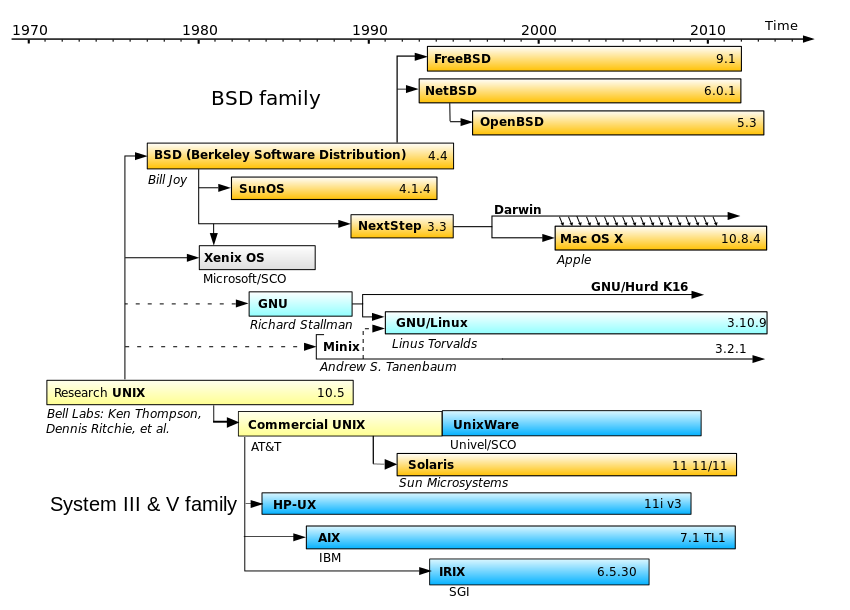
\includegraphics[width=0.9\linewidth]{Unix_timeline.png}
\caption{Historia de Unix}
\label{fig1001}
\end{figure}

Era el año 1991 y Linus Torvalds ,que en aquel entonces era un estudiante de informática de la Universidad de Helsinki, empezó a programar las primeras líneas de código de un sistema operativo(finalmente llamado LINUX ) como una afición y sin poderse imaginar la gran repercusión que traería.
Hubo una primera versión no oficial de Linux 0.01, pero esta solo incluía el comienzo del núcleo, estaba escrita en lenguaje ensamblador y asumía que uno tenía acceso a un sistema Minix para su compilación.
El 5 de octubre de 1991, Linus anuncio la primera versión oficial de Linux (versión 0.02). Con esta versión Linus pudo ejecutar Bash (GNU Bourne Again Shell) y gcc (El compilador GNU de C).Desde aquel entonces se han hecho muchísimas versiones con ayuda de programadores de todo el mundo.
Linux es un sistema operativo compatible con Unix, sus dos características principales y que los diferencian del resto de los sistemas operativos que encontramos en el mercado son:
\begin{itemize}
	\item Es software libre, esto significa que no tenemos que pagar por el uso del mismo.
	\item El sistema viene acompañado del código fuente (el sistema lo forman el núcleo del sistema (kernel) mas un gran numero de librerías que hacen posible su utilización).
\end{itemize}

Las plataformas en las que en un principio se puede utilizar Linux son: Pentium, Pentium Pro, Pentium II/III/IV, Amiga y Atari, también existen versiones para su utilización en otras plataformas, como Alpha, ARM, MIPS, PowerPC y SPARC.
En los últimos tiempos, ciertas casas de software comercial han empezado a distribuir sus productos para Linux y la presencia del mismo en empresas aumenta rápidamente por la excelente relación calidad-precio que se consigue con Linux.



\subsection{Tux}
Tux es el nombre de la mascota oficial de Linux. Creado por Larry Ewing en 1996, es un pequeño pingüino de aspecto risueño y cómico. La idea de que la mascota de kernel Linux fuera un pingüino provino del mismo Linus Torvalds, creador de kernel Linux.
Existen dos versiones sobre el origen de su nombre:
\begin{itemize}
	\item Los pingüinos parecen vestir un     esmoquin (que en inglés es tuxedo max, abreviado tux).
	\item Las letras que componen Tux provienen de las palabras Torvalds y Unix.
\end{itemize}
  
Hay quien dice que Tux era el nombre de un peluche que tenia Linus que era un pingüino llamado Tux.
El logotipo se puede usar y modificar sin restricciones, siempre que se reconozca la autoría de Larry Ewing, ya que es su trabajo y se debe reconocer su autoría tal y como se indica en su página\footnote{La página es http://lewing.org/}.

\begin{figure}
	\centering
	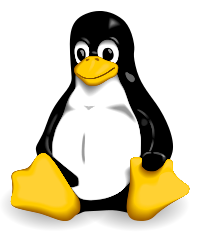
\includegraphics[width=0.5\linewidth]{200px-Tux.png}
	\caption{Símbolo de Linux desarrollado por Larry Ewing}
	\label{fig1002}
\end{figure}

\subsection{Distribuciones de Linux}

Una distribución es un conjunto de aplicaciones reunidas por un grupo, empresa o persona para permitir instalar fácilmente un sistema Linux. En general se destacan por las herramientas para configuración y sistemas de paquetes de software a instalar.
Una distribución no es otra cosa, que una recopilación de programas y ficheros, organizados y preparados para su instalación. Estas distribuciones se pueden obtener a través de Internet, o comprando los CDs de las mismas, los cuales contendrán todo lo necesario para instalar un sistema Linux bastante completo y en la mayoría de los casos un programa de instalación que nos ayudara en la tarea de una primera instalación. Casi todos los principales distribuidores de Linux, ofrecen la posibilidad de bajarse sus distribuciones, via FTP (sin cargo alguno).

Existen muchas y variadas distribuciones creadas por diferentes empresas y organizaciones a unos precios bastantes asequibles (si se compran los CDs, en vez de bajársela via FTP).

A continuación se muestra una gráfica con todas las distribuciones a lo largo de los últimos años. Este gráfico es grande.

\begin{figure}
	\centering
	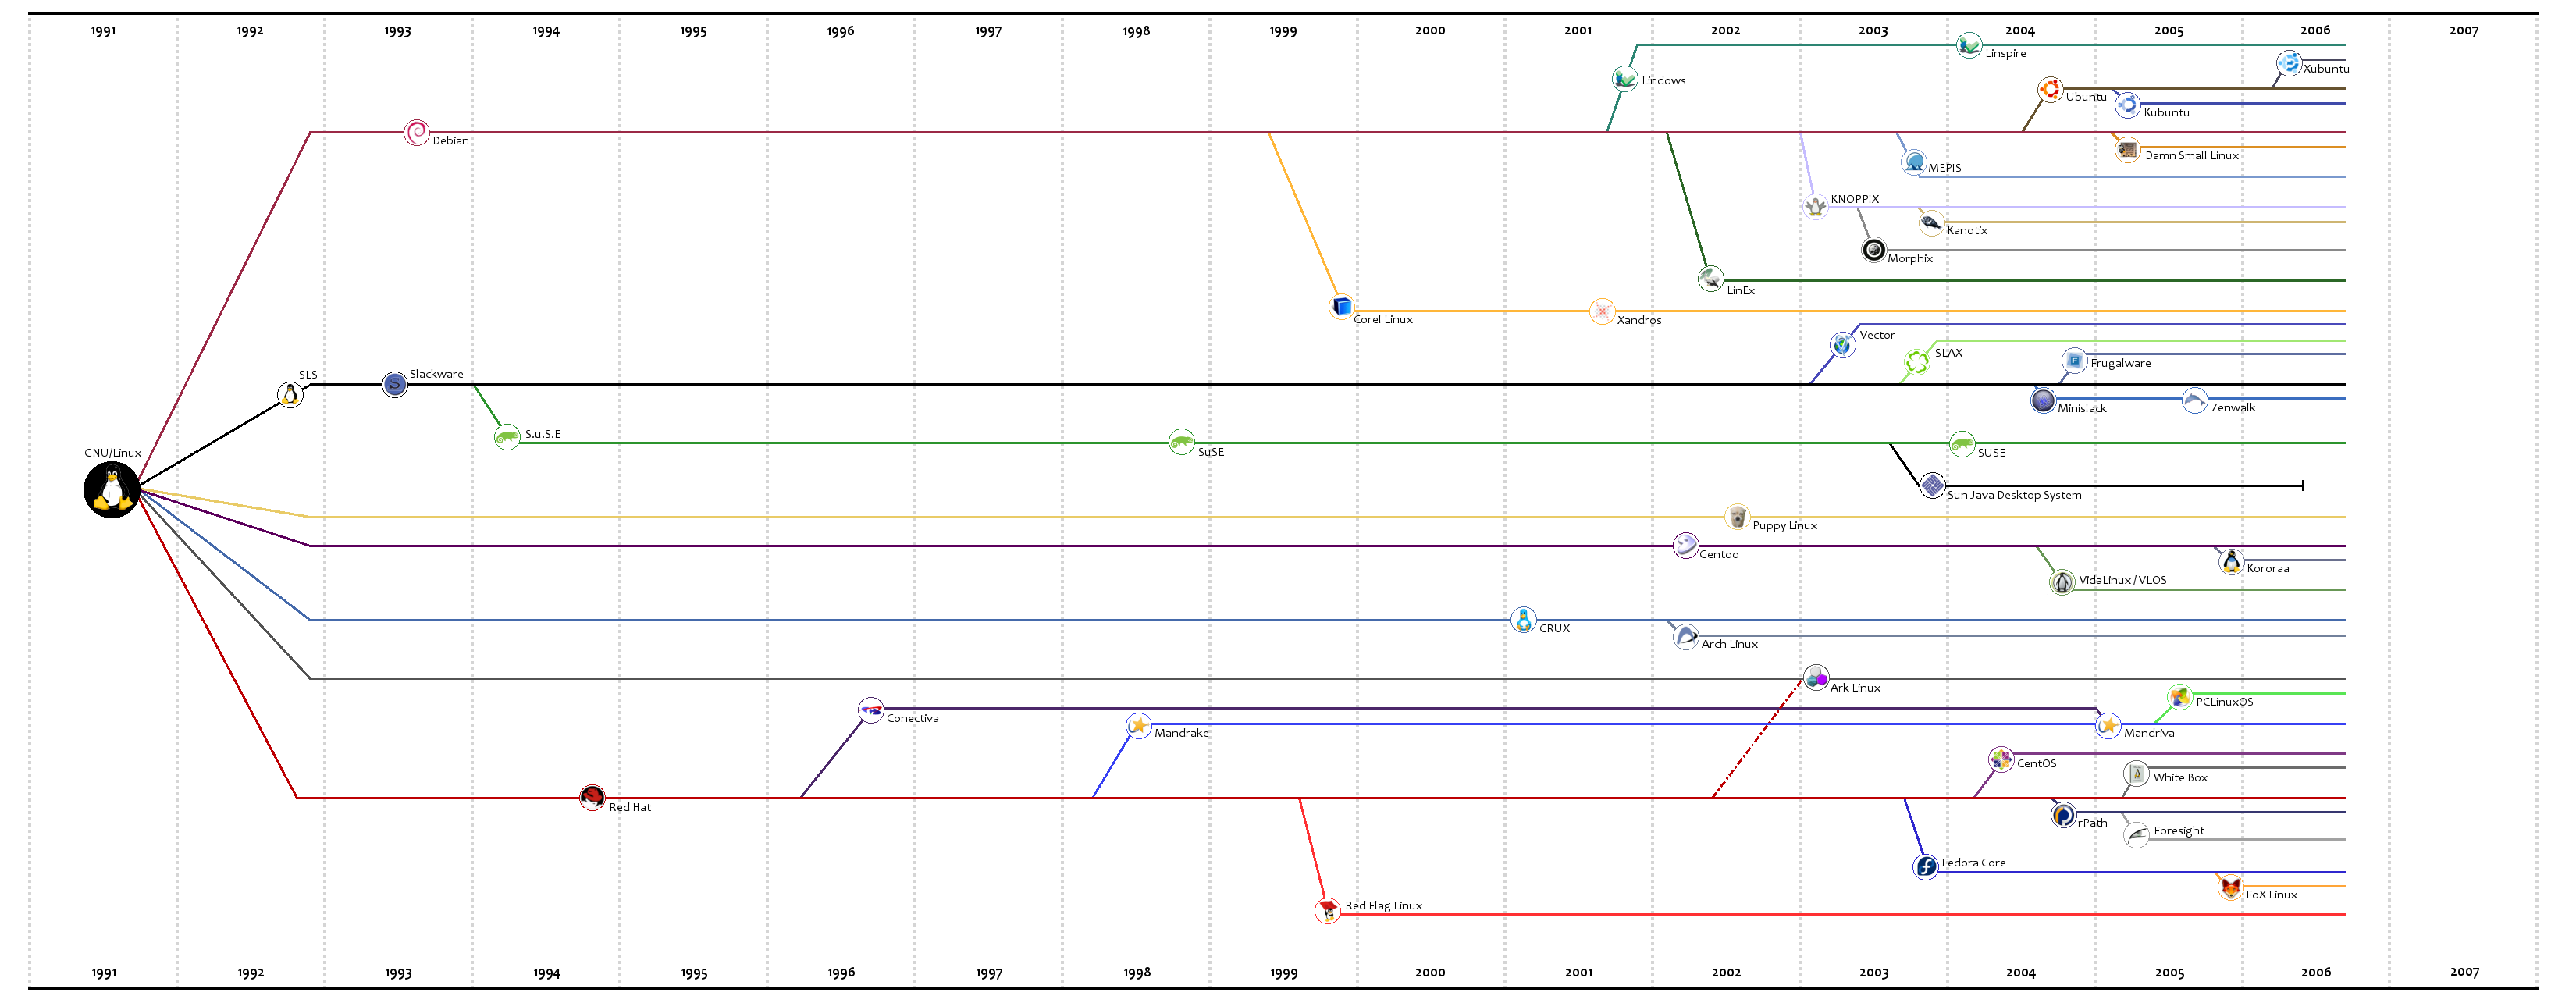
\includegraphics[width=1.0\linewidth]{linux_distros.png}
	\caption{Historia de las Distribuciones de Linux}
	\label{fig1003}
\end{figure}

\section{Virtualización}

En Informática, virtualización es la creación -a través de software- de una versión virtual de algún recurso tecnológico, como puede ser una plataforma de hardware, un sistema operativo, un dispositivo de almacenamiento u otros recursos de red. Dicho de otra manera, se refiere a la abstracción de los recursos de una computadora, llamada Hypervisor o VMM (Virtual Machine Monitor) que crea una capa de abstracción entre el hardware de la máquina física (host) y el sistema operativo de la máquina virtual (virtual machine, guest), dividiéndose el recurso en uno o más entornos de ejecución.

Esta capa de software (VMM) maneja, gestiona y arbitra los cuatro recursos principales de una computadora (CPU, Memoria, Dispositivos Periféricos y Conexiones de Red) y así podrá repartir dinámicamente dichos recursos entre todas las máquinas virtuales definidas en el computador central. Esto hace que se puedan tener varios ordenadores virtuales ejecutándose en el mismo ordenador físico.

Tal término es antiguo; se viene usando desde 1960, y ha sido aplicado a diferentes aspectos y ámbitos de la informática, desde sistemas computacionales completos, hasta capacidades o componentes individuales.

La virtualización se encarga de crear una interfaz externa que encapsula una implementación subyacente mediante la combinación de recursos en localizaciones físicas diferentes, o por medio de la simplificación del sistema de control. Un avanzado desarrollo de nuevas plataformas y tecnologías de virtualización ha hecho que en los últimos años se haya vuelto a prestar atención a este concepto.

La máquina virtual en general simula una plataforma de hardware autónoma incluyendo un sistema operativo completo que se ejecuta como si estuviera instalado. Típicamente varias máquinas virtuales operan en un computador central. Para que el sistema operativo ``guest'' funcione, la simulación debe ser lo suficientemente grande (siempre dependiendo del tipo de virtualización).

\subsection{Virtualización por Sistema Operativo}

Virtualizar significa instalar un sistema operativo dentro de otro al que se le llama anfitrión (HOST), mediante el uso de una máquina virtual. Frecuentemente denominada virtualización compartida del Sistema Operativo o virtualización del SO, la virtualización del Sistema Operativo virtualiza servidores en la capa del sistema operativo (kernel). Este método de virtualización crea particiones aisladas o entornos virtuales (VEs) en un único servidor físico e instancia de SO para así maximizar los esfuerzos de administración del hardware, software y centro de datos. La Virtualización de Hypervisor tiene una capa base (generalmente un kernel, Linux que se muestra aquí como un hypervisor o SO estándar, lo mismo que Windows Server 2008 R2 Hyper-V) que se carga directamente en el servidor base. Para asignar hardware y recursos a las máquinas virtuales (VMs), es recomendable que todo el hardware del servidor esté virtualizado. La siguiente capa superior muestra cada chip, placa, etc. que debe virtualizarse para que así pueda ser asignado a las VMs. Una vez en la VM, hay un copia completa de un sistema operativo y finalmente la aplicación o carga de trabajo.

La Virtualización de SO mejora el rendimiento, gestión y eficiencia. En la base reside un sistema operativo anfitrión estándar, como en el caso de Parallels Virtuozzo que incluye Windows y un sistema con núcleo Linux. A continuación encontramos la capa de virtualización, con un sistema de archivos propietario y una capa de abstracción de servicio de kernel que garantiza el aislamiento y seguridad de los recursos entre distintos contenedores. La capa de virtualización hace que cada uno de los contenedores aparezca como servidor autónomo. Finalmente, el contenedor aloja la aplicación o carga de trabajo.

Virtualizar el sistema operativo es una opción interesante si no queremos instalar dos sistemas operativos en el mismo ordenador, pero si por el contrario lo que hacemos es instalarlo, todos los sistemas operativos que tengamos instalados funcionaran de la misma manera que si estuvieran instalados en distintos ordenadores.

El único y pequeño inconveniente es que necesitamos un gestor de arranque que al encender nuestro ordenador nos dé la opción de elegir qué sistema operativo queremos utilizar, lo que conlleva que si por ejemplo estamos en Windows y queremos cambiar a GNU/Linux deberíamos reiniciar nuestro ordenador. La virtualización por el contrario permite cambiar de sistema operativo como si se tratase de cualquier otro programa, sin embargo, esta agilidad tiene la desventaja de que un sistema operativo virtualizado no es tan potente como uno que ya estuviera instalado \footnote{Tomado de http://es.wikipedia.org/wiki/Virtualización}.

\subsubsection{Software para virtualizar en Windows}

Suponiendo que tu computadora esta utilizando Windows como sistema operativo principal (host), existen dos software que te permiten virtualizar un sistema operativo dentro de windows, estos son: (a) VirtualBox (b) VMware player, ambos software son gratis.

En este curso utilizaremos el software VMWare player. En la figura \ref{fig1004} se puede ver la dirección desde la cual bajar el software.

\begin{figure}
	\centering
	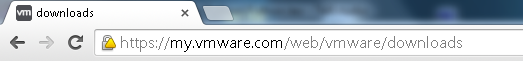
\includegraphics[width=1.0\linewidth]{direccionVMware.png}
	\caption{Dirección donde bajar el VMware Player}
	\label{fig1004}
\end{figure}

En la figura \ref{fig1005} se puede observar el archivo para bajar.

\begin{figure}
	\centering
	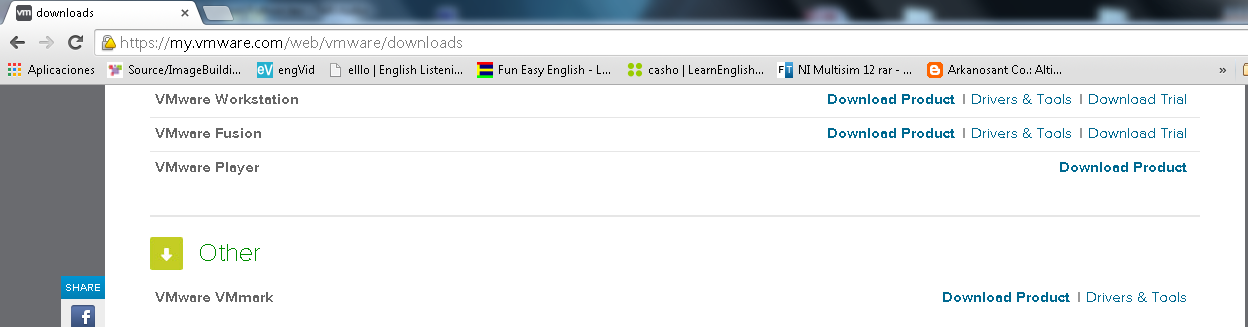
\includegraphics[width=1.0\linewidth]{ArchivoVMware.png}
	\caption{Archivo para bajar VMware Player}
	\label{fig1005}
\end{figure}

\subsubsection{Bajando la distribución de Linux}
Como se ha mencionado existen muchas versiones de linux, para este curso utilizaremos una versión amigable basada en Ubuntu, su nombre es Elementary OS, en enero de 2015 elementary era la séptima distribución mas popular de linux, como se indica en la \ref{fig1006}.

\begin{figure}
	\centering
	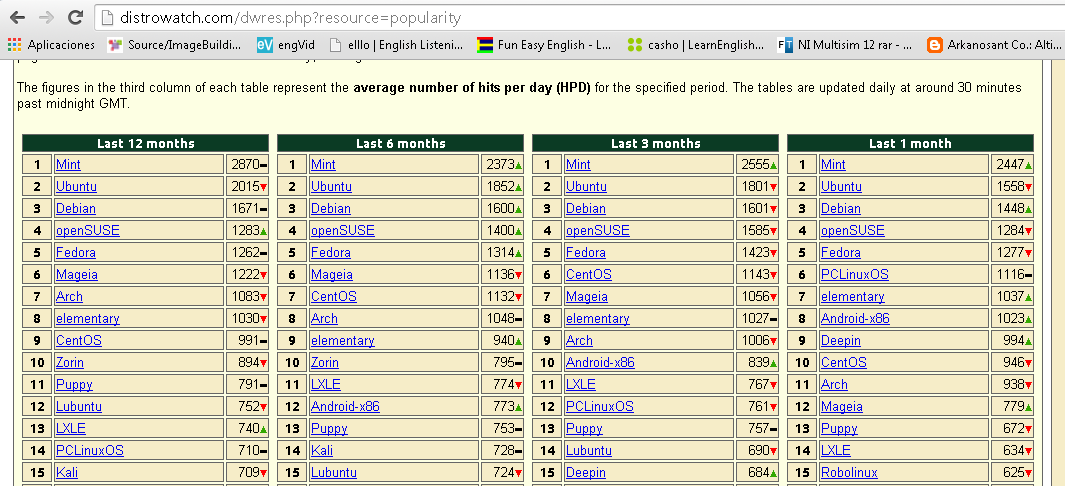
\includegraphics[width=1.0\linewidth]{DistroWatchEnero2015.png}
	\caption{Distrubuciones de Linux mas exitosas segun el sitio DistroWatch en enero 2015}
	\label{fig1006}
\end{figure}

Es necesario bajar el archivo .iso de la distribución de linux que se desea virtualizar, en nuestro caso en la figura \ref{fig1007} se muestra la dirección. Elementary es una distribución de linux basado en Ubuntu, que no tiene fechas fijas de actualizaciones y es un proyecto de reciente creación desarrollado por voluntarios en canada y otras partes del mundo.

\begin{figure}
	\centering
	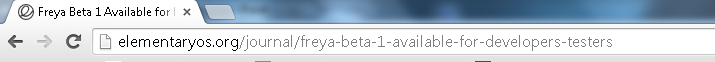
\includegraphics[width=1.0\linewidth]{elementaryOS.png}
	\caption{Dirección desde donde debe bajarse la Elementary OS en su nueva versión Freya Beta 1}
	\label{fig1007}
\end{figure}

La razón de utilizar esta versión de Linux es debido a que se esta desarrollando software y/o modificando software específico para el ambiente de la distribución, aún cuando los conceptos visuales son una copia del OSX de la mac. Los tiempos de actualización de la distribución aún son lentos y su grupo de desarrollo aún es pequeño, en pocas palabras es un proyecto naciente pero con gran potencial. 

\begin{figure}
	\centering
	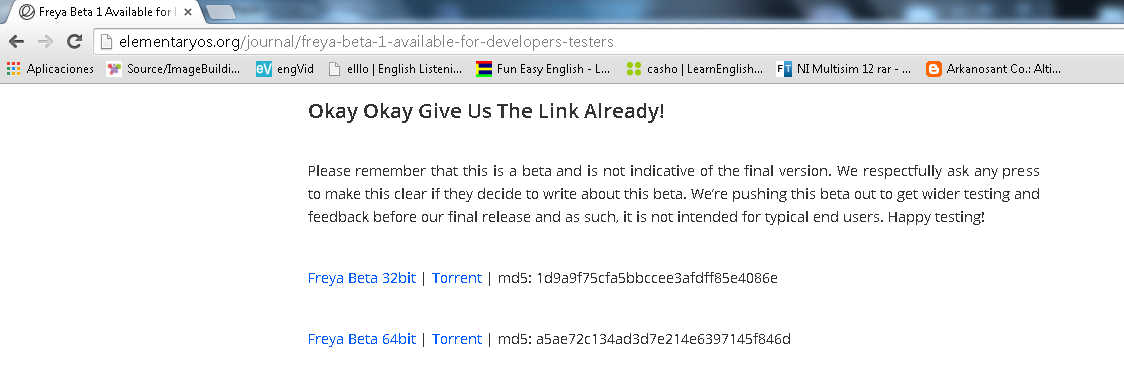
\includegraphics[width=1.0\linewidth]{ArchivoElementaryOS.png}
	\caption{Opciones de archivos para bajar de Elementary OS en su nueva versión Freya Beta 1}
	\label{fig1008}
\end{figure}

En la figura \ref{fig1008} se puede observar las dos versiones para bajar elementary Freya Beta 1, que es la versión de 32 bits y la de 64 bits, según las características de su computadora y según si tienen o no activada la virtualización por hardware en el setup de su computadora.

\section{Creando una máquina virtual con VMware Player}
	
\begin{figure}
	\centering
	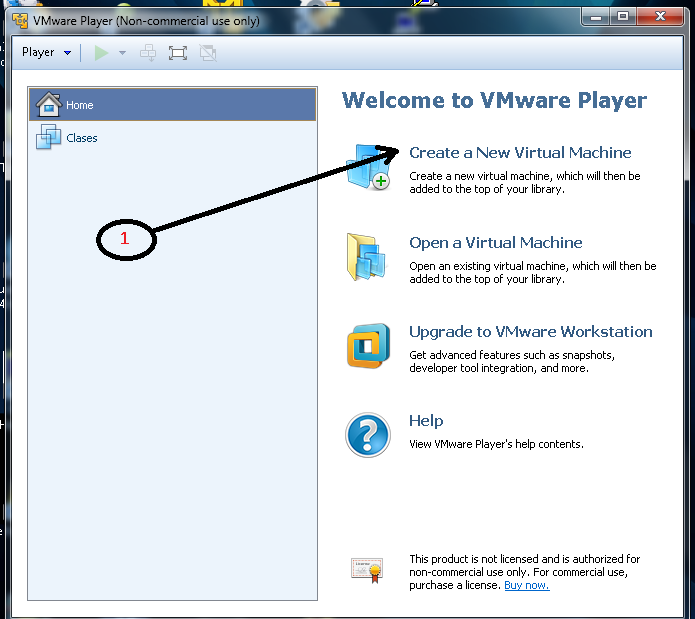
\includegraphics[width=1.0\linewidth]{VMwarePlayerInicio.png}
	\caption{Inicio del VMWare Player}
	\label{fig1009}
\end{figure}

En la figura \ref{fig1009} se muestra la pantalla de inicio del software VMWare Player. En la figura \ref{fig1009} se puede observar el número 1 encerrado en una elipse con lo cual se indica que el primer paso es dar click sobre la opción \textbf{Create a New Virtual Machine}.


\begin{figure}
	\centering
	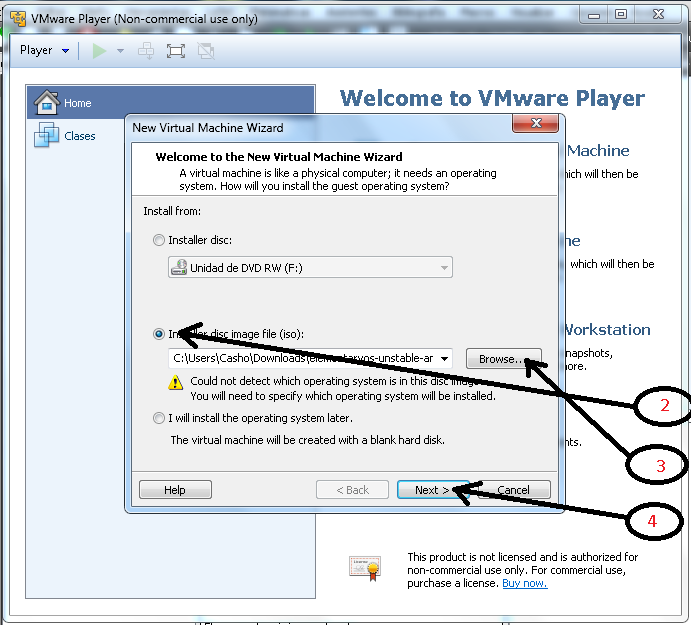
\includegraphics[width=1.0\linewidth]{VMwarePlayer2y3.png}
	\caption{Enlace de la maquina virtual con el archivo de arranque de linux}
	\label{fig1010}
\end{figure}


En la figura \ref{fig1010} se enlaza la máquina virtual con la distribución de linux que se le instalará, en el paso dos se le indica que el archivo que se usará será un archivo iso y en el paso 3 se busca ese archivo en la computadora. Y posteriormente se da click en el boton next.


\begin{figure}
	\centering
	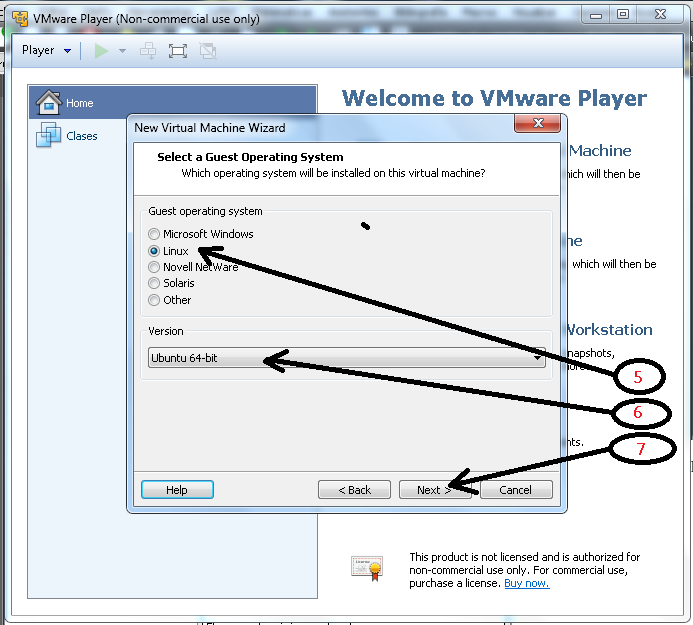
\includegraphics[width=1.0\linewidth]{VMwarePlayer5y6y7.png}
	\caption{Características del Sistema Operativo Invitado}
	\label{fig1011}
\end{figure}

En la figura \ref{fig1011} se muestran los pasos 5, 6 y 7. En el paso 5 se muestra el sistema GUEST seleccionado, en este caso será \textbf{Linux}, en el paso 6 se eligirá  la versión que debe ser ubuntu y el número de bits coincidir con la versión del número de bits bajado del archivo linux. En el paso 7 se da next.

\begin{figure}
	\centering
	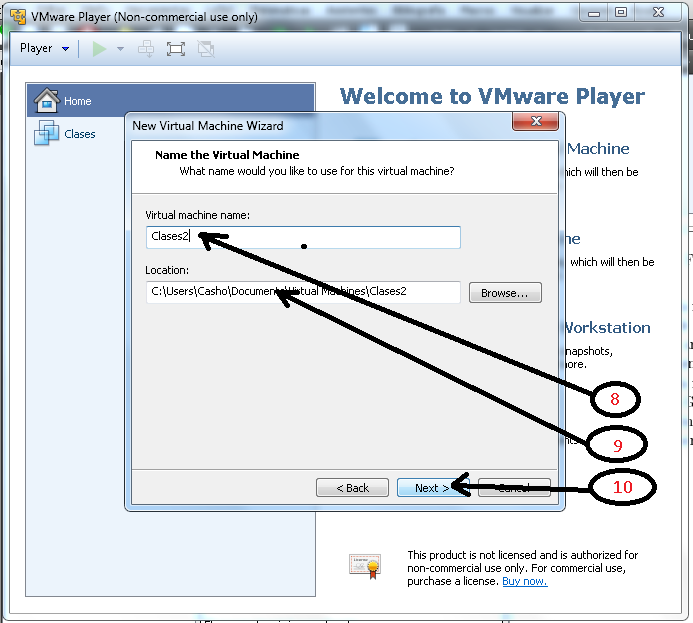
\includegraphics[width=1.0\linewidth]{VMwarePlayer8y9y10.png}
	\caption{Nombre de la máquina virtual}
	\label{fig1012}
\end{figure}
  
En la figura \ref{fig1012} se pueden ver los pasos 8 (donde se establece el nombre de la maquina virtual), el paso 9 donde se establece la carpeta donde se guardará el archivo, en el paso 10 se da click en el botón next.

\begin{figure}
	\centering
	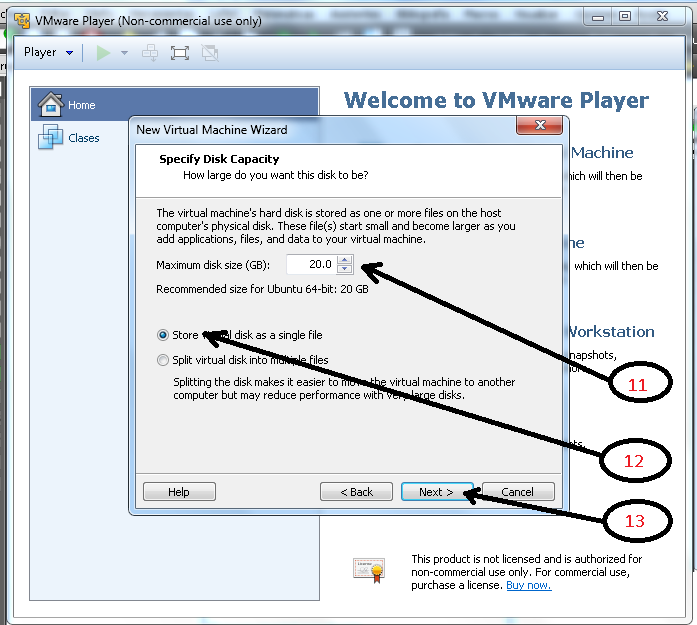
\includegraphics[width=1.0\linewidth]{VMwarePlayer11y12y13.png}
	\caption{Tamaño de la Máquina Virtual}
	\label{fig1013}
\end{figure}
En la figura \ref{fig1013} se muestran los paso 11 (en donde se elige el tamaño de la máquina virtual), en el paso 12 se graba toda la máquina virtual en un solo archivo, y en el paso 13 se da click en next.

Después de lo cual se da click en el boton finish.

Después de lo cual se da \textbf{play} en la máquina virtual y se instala el sistema operativo siguiendo los pasos que se indican.

Al terminar de instalar la máquina virtual, se debe desenlazar el archivo iso con la máquina virtual.

\begin{figure}
	\centering
	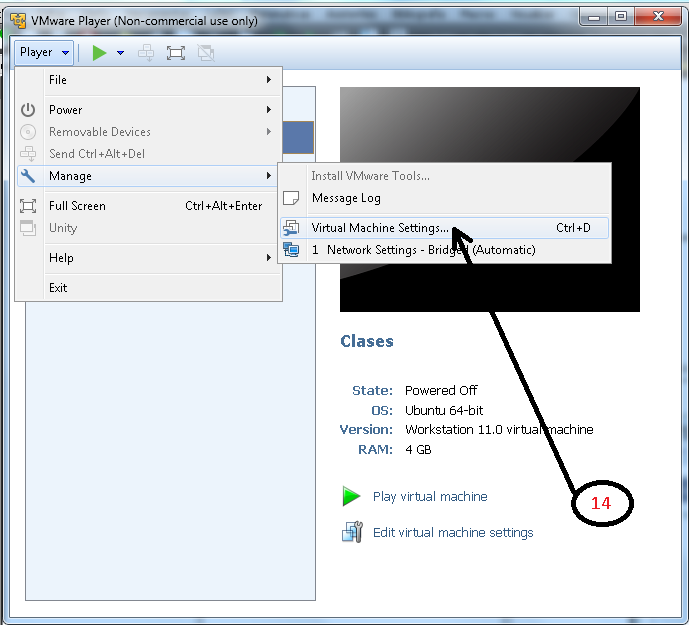
\includegraphics[width=1.0\linewidth]{VMwarePlayer14.png}
	\caption{Características de la Máquina Virtual}
	\label{fig1014}
\end{figure}

\begin{figure}
	\centering
	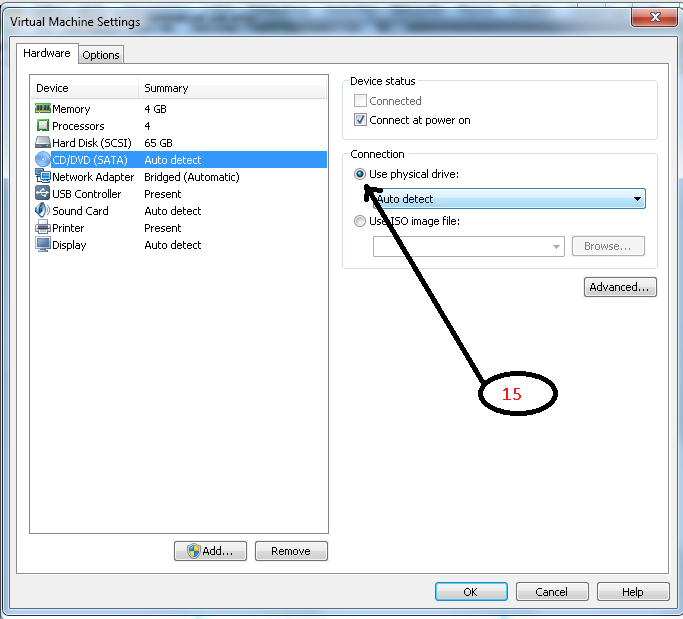
\includegraphics[width=1.0\linewidth]{VMwarePlayerFin.png}
	\caption{Desacoplar el disco iso de la máquina virtual}
	\label{fig1015}
\end{figure}

En la figura \ref{fig1015} se muestra la opción a seleccionar para desacoplar el iso de la máquina virtual para poder correrla sin volver a instalar el sistema operativo.

\chapter{Instalando Python y el IDE para la programación}

Cuando compilamos un programa escrito en C o en Fortran generamos un ejecutable. Para hacer funcionar ese ejecutable nos basta con muy poca cosa; en el caso de un ``hola, mundo'' basta con simplemente ejecutarlo. El sistema operativo lo considera ejecutable y simplemente cumple sus ordenes.

Esto no sucede así en los lenguajes interpretados. El código en Python nunca llega a traducirse a algo que el sistema operativo pueda entender. En Python el programa termina convertido en un ensamblador propio que una máquina virtual es capaz de entender y ejecutar. La consecuencia principal de este método es que es imprescindible contar con un intérprete de Python instalado en el ordenador para poder ejecutar código en Python.

Esta no es hoy en día una condición demasiado severa. El único sistema operativo mayoritario que no cuenta con un intérprete de Python instalado por omisión es Windows. Linux, Mac OSX, Solaris y AIX entre otros cuentan con uno, aunque algunas veces compensa instalar una versión más actualizada que la que encontraremos en la distribución del sistema operativo. En el caso especial de Windows bastará con descargarse un instalador, darle doble clic y decir que sí a todo.

Cuando ejecutamos código en Python lo lanzamos a un intérprete que es capaz de entender este lenguaje. A diferencia de los lenguajes estáticos como C o Fortran en el que un compilador convierte el código de programa en un ejecutable que el sistema operativo es capaz de entender.

\section{Instalando Eclipse}

Eclipse es un programa informático compuesto por un conjunto de herramientas de programación de código abierto multiplataforma para desarrollar lo que el proyecto llama "Aplicaciones de Cliente Enriquecido", opuesto a las aplicaciones "Cliente-liviano" basadas en navegadores. Esta plataforma, típicamente ha sido usada para desarrollar entornos de desarrollo integrados (del inglés IDE), como el IDE de Java llamado Java Development Toolkit (JDT) y el compilador (ECJ) que se entrega como parte de Eclipse (y que son usados también para desarrollar el mismo Eclipse). Sin embargo, también se puede usar para otros tipos de aplicaciones cliente, como BitTorrent o Azureus.

Eclipse es también una comunidad de usuarios, extendiendo constantemente las áreas de aplicación cubiertas. Un ejemplo es el recientemente creado Eclipse Modeling Project, cubriendo casi todas las áreas de Model Driven Engineering.

Eclipse fue desarrollado originalmente por IBM como el sucesor de su familia de herramientas para VisualAge. Eclipse es ahora desarrollado por la Fundación Eclipse, una organización independiente sin ánimo de lucro que fomenta una comunidad de código abierto y un conjunto de productos complementarios, capacidades y servicios.

Eclipse fue liberado originalmente bajo la Common Public License, pero después fue re-licenciado bajo la Eclipse Public License. La Free Software Foundation ha dicho que ambas licencias son licencias de software libre, pero son incompatibles con Licencia pública general de GNU (GNU GPL)

\section{Pasos para instalar eclipse en Elementary OS}

\subsection{Paso 1}
Primero en el Desktop de Elementary OS dar click en aplicaciones, figura \ref{fig1016}.

\begin{figure}
	\centering
	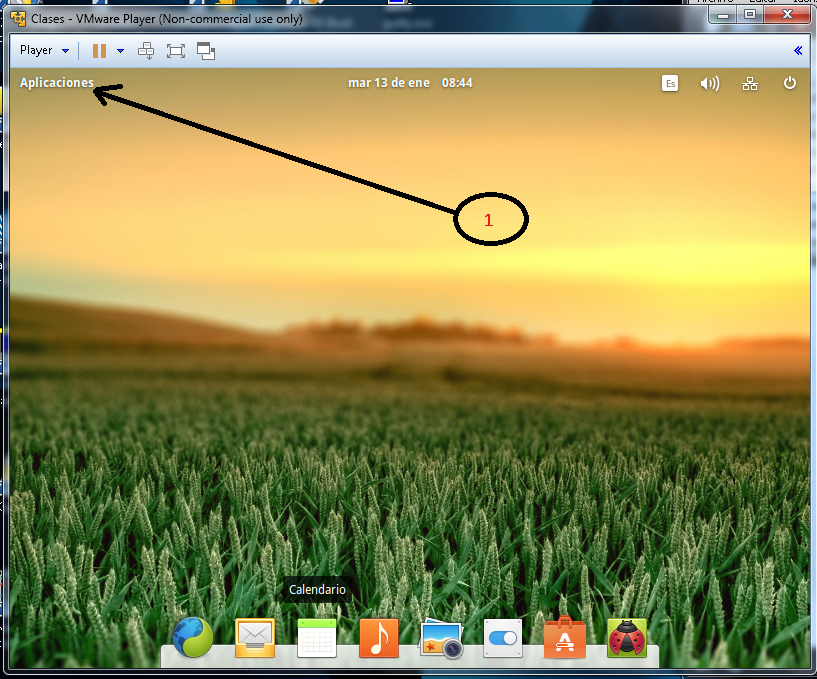
\includegraphics[width=0.5\linewidth]{Eclipse1.png}
	\caption{Desktop de Elementary OS}
	\label{fig1016}
\end{figure}


\subsection{Paso 2 y Paso 3}

Buscar en las aplicaciones de Elementary OS el centro de Software y dar click en el, figura \ref{fig1017}.

\begin{figure}
	\centering
	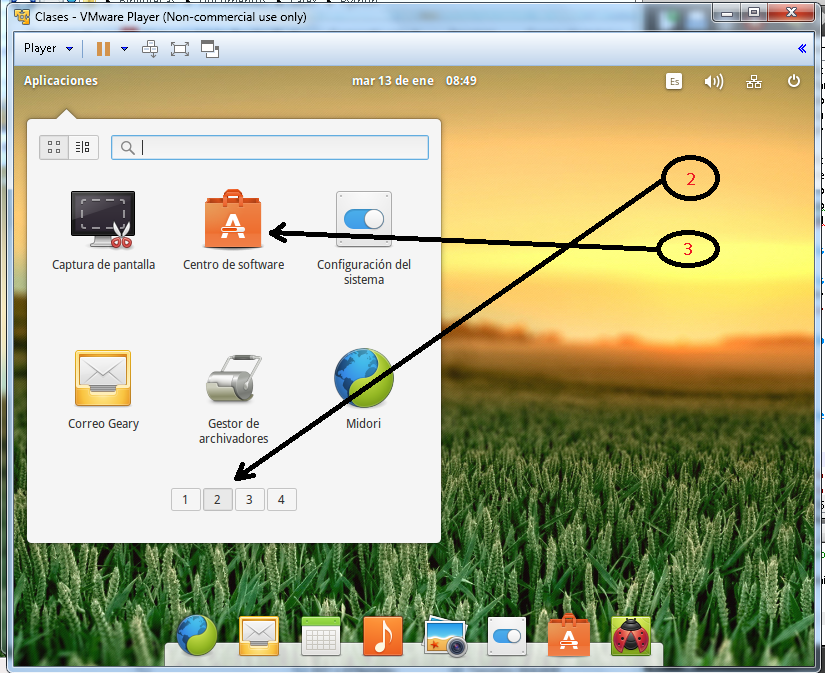
\includegraphics[width=0.5\linewidth]{Eclipse2y3.png}
	\caption{Aplicaciones de Elementary OS}
	\label{fig1017}
\end{figure}


\subsection{Paso 4 y paso 5}

Cuando abre la aplicación de centro de software, introducir el nombre eclipse en el buscador y posteriormente dar click en instalar, como se indica en la figura

\begin{figure}
	\centering
	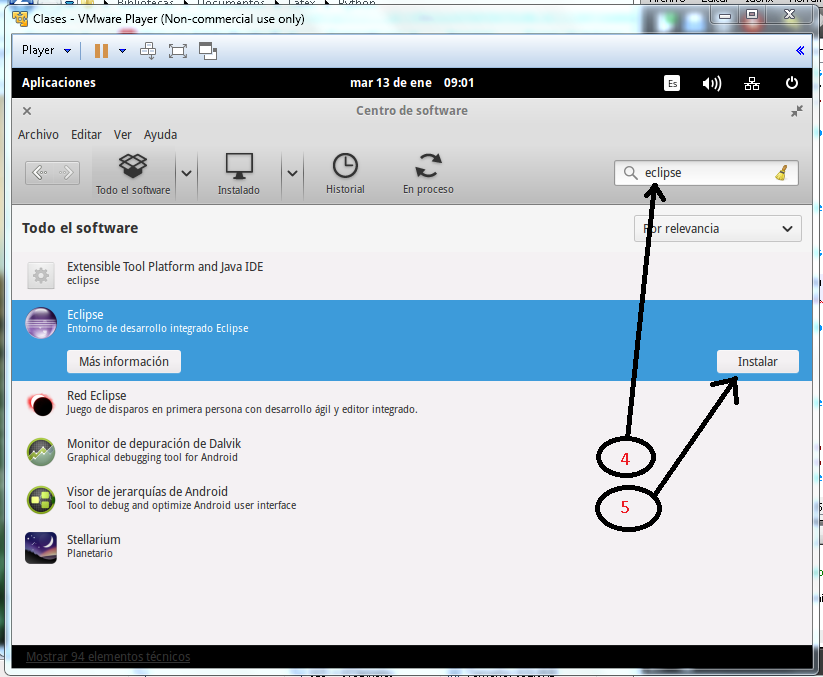
\includegraphics[width=0.5\linewidth]{Eclipse4y5.png}
	\caption{Centro de Software}
	\label{fig1018}
\end{figure}

Antes de iniciar la instalación te pedirá el \textbf{password} de tu cuenta, solo hay que introducirla y darle \textbf{enter} para que inicie la instalación

\section{Instalando PyDev}

Para instalar PyDev a las extensiones de PyDev se debe utilizar el \textbf{Eclipse Update Manager}, para ello es necesario ir a la opción del menu \textbf{help>Install New Software}, como se muestra \ref{fig1019}.

\begin{figure}
	\centering
	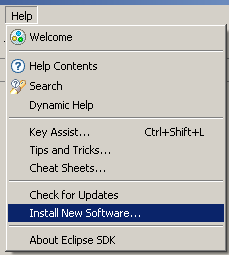
\includegraphics[width=0.5\linewidth]{Pydev1.png}
	\caption{Menu de ayuda de eclipse}
	\label{fig1019}
\end{figure}

En la figura \ref{fig1020} se observa la ventana que se despliega, como la figura lo muestra hay que darle click al boton add e introducir el nombre y la dirección que allí se indican.
\begin{figure}
	\centering
	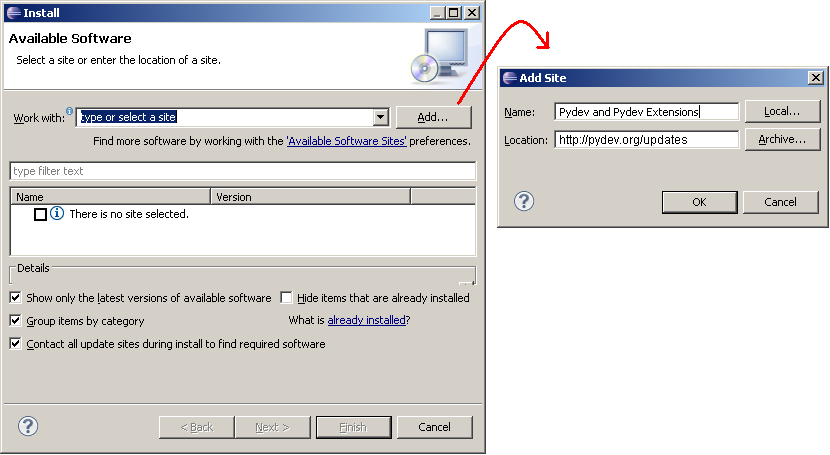
\includegraphics[width=1.0\linewidth]{Pydev2.png}
	\caption{Menu de ayuda de eclipse}
	\label{fig1020}
\end{figure}

Hay muchos sitios para bajar y actualizar el software, en la figura \ref{fig1021}, se muestra las opciones a seleccionar. La Opción \textbf{Work with} debe elegirse \textbf{--All available Sites--}

\begin{figure}
	\centering
	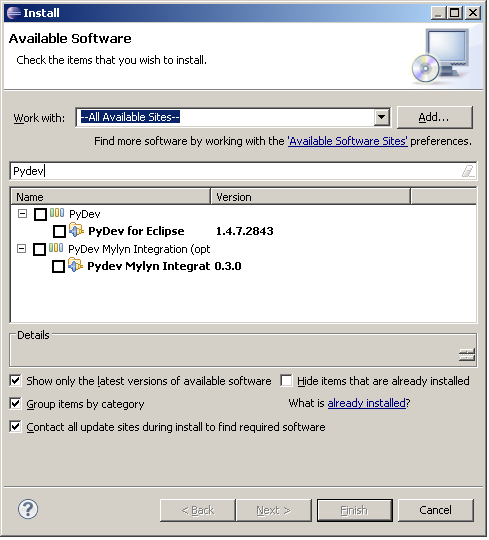
\includegraphics[width=1.0\linewidth]{Pydev3.png}
	\caption{Menu de ayuda de eclipse}
	\label{fig1021}
\end{figure}

Posteriormente debe seleccionar \textbf{next}, y posteriormente next y por último finish, como se indican en la figura \ref{fig1022}, figura \ref{fig1023}.

\begin{figure}
	\centering
	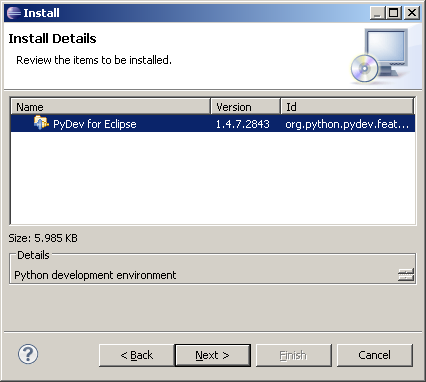
\includegraphics[width=1.0\linewidth]{Pydev4.png}
	\caption{Menu de ayuda de eclipse}
	\label{fig1022}
\end{figure}

\begin{figure}
	\centering
	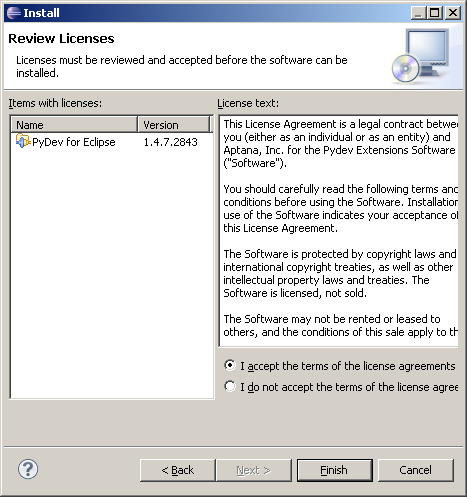
\includegraphics[width=1.0\linewidth]{Pydev5.png}
	\caption{Menu de ayuda de eclipse}
	\label{fig1023}
\end{figure}

\chapter{Introducción a Python}


Para entender este paradigma primero tenemos que comprender qué es una clase y qué es un objeto. Un objeto es una entidad que agrupa un estado y una funcionalidad relacionadas. El estado del objeto se define a través de variables llamadas atributos, mientras que la funcionalidad se modela a través de funciones a las que se les conoce con el nombre de métodos del objeto.
Un ejemplo de objeto podría ser un coche, en el que tendríamos atributos como la marca, el número de puertas o el tipo de carburante y métodos como arrancar y parar. O bien cualquier otra combinación de atributos y métodos según lo que fuera relevante para nuestro programa.

Una clase, por otro lado, no es más que una plantilla genérica a partir de la cuál instanciar los objetos; plantilla que es la que define qué atributos y métodos tendrán los objetos de esa clase.

Volviendo a nuestro ejemplo: en el mundo real existe un conjunto de objetos a los que llamamos coches y que tienen un conjunto de atributos comunes y un comportamiento común, esto es a lo que llamamos clase. Sin embargo, mi coche no es igual que el coche de mi vecino, y aunque pertenecen a la misma clase de objetos, son objetos distintos.

En Python las clases se definen mediante la palabra clave \textit{\textbf{class}} seguida del nombre de la clase, dos puntos (:) y a continuación, indentado, el cuerpo de la clase. Como en el caso de las funciones, si la primera línea del cuerpo se trata de una cadena de texto, esta será la cadena de documentación de la clase o docstring.

\begin{lstlisting}[language=Python]
class Coche:
   """Abstraccion de los objetos coche."""
   def __init__(self, gasolina):
     self.gasolina = gasolina
     print ("Tenemos", gasolina, "litros")
		
   def arrancar(self):
      if self.gasolina > 0:
         print ("Arranca")
      else:
         print ("No arranca")
   def conducir(self):
      if self.gasolina > 0:
         self.gasolina -= 1
         print ("Quedan", self.gasolina, "litros")
      else:
         print ("No se mueve")
\end{lstlisting}


Lo primero que llama la atención en el ejemplo anterior es el nombre tan curioso que tiene el método \_\_init\_\_. Este nombre es una convención y no un capricho. El método \_\_init\_\_, con una doble barra baja al principio y final del nombre, se ejecuta justo después de crear un nuevo objeto a partir de la clase, proceso que se conoce con el nombre de instanciación. El método \_\_init\_\_ sirve, como sugiere su nombre, para realizar cualquier proceso de inicialización que sea necesario.

Como vemos el primer parámetro de  \_\_init\_\_ y del resto de métodos de la clase es siempre \textit{\textbf{self}}. Esta es una idea inspirada en Modula-3 y sirve para referirse al objeto actual. Este mecanismo es necesario para poder acceder a los atributos y métodos del objeto diferenciando, por ejemplo, una variable local \textbf{mi\_var} de un atributo del objeto \textbf{self.mi\_var}.

Si volvemos al método \_\_init\_\_ de nuestra clase Coche veremos cómo se utiliza \textbf{\textit{self}} para asignar al atributo gasolina del objeto (self.gasolina) el valor que el programador especificó para el parámetro gasolina. El parámetro gasolina se destruye al final de la función, mientras que el atributo gasolina se conserva (y puede ser accedido) mientras el objeto viva.


Para crear un objeto se escribiría el nombre de la clase seguido de cualquier parámetro que sea necesario entre paréntesis. Estos parámetros son los que se pasarán al método \_\_init\_\_, que como decíamos es el método que se llama al instanciar la clase.

\begin{lstlisting}[language=Python]
mi_coche = Coche(3)
\end{lstlisting}

Te preguntarás entonces cómo es posible que a la hora de crear nuestro primer objeto pasemos un solo parámetro a \_\_init\_\_, el número 3, cuando la definición de la función indica claramente que precisa de dos parámetros (self y gasolina). Esto es así porque Python pasa el primer argumento (la referencia al objeto que se crea) automágicamente.

Ahora que ya hemos creado nuestro objeto, podemos acceder a sus atributos y métodos mediante la sintaxis \textbf{objeto.atributo} y \textbf{objeto.metodo()}:

\begin{lstlisting}[language=Python]
>>> print mi_coche.gasolina
3
>>> mi_coche.arrancar()
Arranca
>>> mi_coche.conducir()
Quedan 2 litros
>>> mi_coche.conducir()
Quedan 1 litros
>>> mi_coche.conducir()
Quedan 0 litros
>>> mi_coche.conducir()
No se mueve
>>> mi_coche.arrancar()
No arranca
>>> print mi_coche.gasolina
0
\end{lstlisting}

Como último apunte recordar que en Python, como ya se comentó en repetidas ocasiones anteriormente, todo son objetos. Las cadenas, por ejemplo, tienen métodos como upper(), que devuelve el texto en mayúsculas o count(sub), que devuelve el número de veces que se encontró la cadena sub en el texto.

\section{Herencia}

Hay tres conceptos que son básicos para cualquier lenguaje de programación orientado a objetos: el encapsulamiento, la herencia y el polimorfismo.

En un lenguaje orientado a objetos cuando hacemos que una clase (subclase) herede de otra clase (superclase) estamos haciendo que la subclase contenga todos los atributos y métodos que tenía la superclase. No obstante al acto de heredar de una clase también se le llama a menudo ``extender una clase''.


Supongamos que queremos modelar los instrumentos musicales de una banda, tendremos entonces una clase Guitarra, una clase Batería, una clase Bajo, etc. Cada una de estas clases tendrá una serie de atributos y métodos, pero ocurre que, por el mero hecho de ser instrumentos musicales, estas clases compartirán muchos de sus atributos y métodos; un ejemplo sería el método tocar().

Es más sencillo crear un tipo de objeto Instrumento con las atributos y métodos comunes e indicar al programa que Guitarra, Batería y Bajo son tipos de instrumentos, haciendo que hereden de Instrumento.

Para indicar que una clase hereda de otra se coloca el nombre de la clase de la que se hereda entre paréntesis después del nombre de la clase:

\begin{lstlisting}[language=Python]
class Instrumento:
   def __init__(self, precio):
      self.precio = precio
   def tocar(self):
      print ("Estamos tocando musica")
   def romper(self):
      print ("Eso lo pagas tu")
      print ("Son", self.precio, "$$$")
class Bateria(Instrumento):
   pass
class Guitarra(Instrumento):
   pass
\end{lstlisting}

Como Bateria y Guitarra heredan de Instrumento, ambos tienen un método tocar() y un método romper(), y se inicializan pasando un parámetro precio. Pero, ¿qué ocurriría si quisiéramos especificar un nuevo parámetro tipo\_cuerda a la hora de crear un objeto Guitarra? Bastaría con escribir un nuevo método \_\_init\_\_ para la clase Guitarra que se ejecutaría en lugar del \_\_init\_\_ de Instrumento. Esto es lo que se conoce como sobreescribir métodos.

Ahora bien, puede ocurrir en algunos casos que necesitemos sobreescribir un método de la clase padre, pero que en ese método queramos ejecutar el método de la clase padre porque nuestro nuevo método no necesite más que ejecutar un par de nuevas instrucciones extra. En ese caso usaríamos la sintaxis SuperClase.metodo(self, args) para llamar al método de igual nombre de la clase padre. Por ejemplo, para llamar al método \_\_init\_\_ de Instrumento desde Guitarra usaríamos Instrumento.\_\_init\_\_(self, precio). Observa que en este caso si es necesario especificar el parámetro \textbf{\textit{self}}.

\section{Herencia Múltiple}

En Python, a diferencia de otros lenguajes como Java o C\#, se permite la herencia múltiple, es decir, una clase puede heredar de varias clases a la vez. Por ejemplo, podríamos tener una clase Cocodrilo que heredara de la clase Terrestre, con métodos como caminar() y atributos como velocidad\_caminar y de la clase Acuatico, con métodos como nadar() y atributos como velocidad\_nadar. Basta con enumerar las clases de las que se hereda separándolas por comas:

\begin{lstlisting}[language=Python]
class Cocodrilo(Terrestre, Acuatico):
   pass
\end{lstlisting}

En el caso de que alguna de las clases padre tuvieran métodos con el mismo nombre y número de parámetros las clases sobreescribirían la implementación de los métodos de las clases más a su derecha en la definición.

En el siguiente ejemplo, como Terrestre se encuentra más a la izquierda, sería la definición de desplazar de esta clase la que prevalecería, y por lo tanto si llamamos al método desplazar de un objeto de tipo Cocodrilo lo que se imprimiría sería ``El animal anda".

\begin{lstlisting}[language=Python]
class Terrestre:
   def desplazar(self):
      print ("El animal anda")
class Acuatico:
   def desplazar(self):
      print ("El animal nada")
class Cocodrilo(Terrestre, Acuatico):
   pass
c = Cocodrilo()
c.desplazar()
\end{lstlisting}

\section{Polimorfismo}

La palabra polimorfismo, del griego \textit{poly morphos} (varias formas), se refiere a la habilidad de objetos de distintas clases de responder al mismo mensaje. Esto se puede conseguir a través de la herencia: un objeto de una clase derivada es al mismo tiempo un objeto de la clase padre, de forma que allí donde se requiere un objeto de la clase padre también se puede utilizar uno de la clase hija.
Python, al ser de tipado dinámico, no impone restricciones a los tipos que se le pueden pasar a una función, por ejemplo, más allá de que el objeto se comporte como se espera: si se va a llamar a un método f() del objeto pasado como parámetro, por ejemplo, evidentemente el objeto tendrá que contar con ese método. Por ese motivo, a diferencia de lenguajes de tipado estático como Java o C++, el polimorfismo en Python no es de gran importancia.

En ocasiones también se utiliza el término polimorfismo para referirse a la sobrecarga de métodos, término que se define como la capacidad del lenguaje de determinar qué método ejecutar de entre varios métodos con igual nombre según el tipo o número de los parámetros que se le pasa. En Python no existe sobrecarga de métodos (el último método sobreescribiría la implementación de los anteriores), aunque se puede conseguir un comportamiento similar recurriendo a funciones con valores por defecto para los parámetros o a la sintaxis \textbf{*params} o \textbf{**params} explicada en el capítulo sobre las funciones en Python, o bien usando decoradores (mecanismo que veremos más adelante).

\section{Encapsulación}

La encapsulación se refiere a impedir el acceso a determinados métodos y atributos de los objetos estableciendo así qué puede utilizarse desde fuera de la clase.
Esto se consigue en otros lenguajes de programación como Java utilizando modificadores de acceso que definen si cualquiera puede acceder a esa función o variable (public) o si está restringido el acceso a la propia clase (private).

En Python no existen los modificadores de acceso, y lo que se suele hacer es que el acceso a una variable o función viene determinado por su nombre: si el nombre comienza con dos guiones bajos (y no termina también con dos guiones bajos) se trata de una variable o función privada, en caso contrario es pública. Los métodos cuyo nombre comienza y termina con dos guiones bajos son métodos especiales que Python llama automáticamente bajo ciertas circunstancias.

En el siguiente ejemplo sólo se imprimirá la cadena correspondiente al método publico(), mientras que al intentar llamar al método \_\_privado() Python lanzará una excepción quejándose de que no existe (evidentemente existe, pero no lo podemos ver porque es privado).


\begin{lstlisting}[language=Python]
class Ejemplo:
   def publico(self):
      print ("Publico")
   def __privado(self):
      print ("Privado")
ej = Ejemplo()
ej.publico()
ej.__privado()
\end{lstlisting}

Este mecanismo se basa en que los nombres que comienzan con un doble guión bajo se renombran para incluir el nombre de la clase (característica que se conoce con el nombre de \textit{name mangling}). Esto implica que el método o atributo no es realmente privado, y podemos acceder a él mediante una pequeña trampa:

\begin{lstlisting}[language=Python]
ej._Ejemplo__privado()
\end{lstlisting}

En ocasiones también puede suceder que queramos permitir el acceso a algún atributo de nuestro objeto, pero que este se produzca de forma controlada. Para esto podemos escribir métodos cuyo único cometido sea este, métodos que normalmente, por convención, tienen nombres como getVariable y setVariable; de ahí que se conozcan también con el nombre de \textit{getters} y \textit{setters}.

\begin{lstlisting}[language=Python]
class Fecha():
   def __init__(self):
      self.__dia = 1
   def getDia(self):
      return self.__dia
   def setDia(self, dia):
      if dia > 0 and dia < 31:
         self.__dia = dia
      else:
         print ("Error")
mi_fecha = Fecha()
mi_fecha.setDia(33)
\end{lstlisting}


Esto se podría simplificar mediante propiedades, que abstraen al usuario del hecho de que se está utilizando métodos entre bambalinas para obtener y modificar los valores del atributo:


\begin{lstlisting}[language=Python]
class Fecha(object):
   def __init__(self):
      self.__dia = 1
   def getDia(self):
      return self.__dia
   def setDia(self, dia):
      if dia > 0 and dia < 31:
         self.__dia = dia
      else:
         print ("Error")
   dia = property(getDia, setDia)
mi_fecha = Fecha()
mi_fecha.dia = 33
\end{lstlisting}

\section{Clases mejoradas}

En el ejemplo anterior os habrá llamado la atención el hecho de que la clase Fecha derive de object. La razón de esto es que para poder usar propiedades la clase tiene que ser de “nuevo-estilo”, clases enriquecidas introducidas en Python 2.2 que serán el estándar en Python 3.0 pero que aún conviven con las clases “clásicas” por razones de retrocompatibilidad. Además de las propiedades las clases de nuevo estilo añaden otras funcionalidades como descriptores o métodos estáticos.

Para que una clase sea de nuevo estilo es necesario, por ahora, que extienda una clase de nuevo-estilo. En el caso de que no sea necesario heredar el comportamiento o el estado de ninguna clase, como en nuestro ejemplo anterior, se puede heredar de object, que es un objeto vacio que sirve como base para todas las clases de nuevo estilo.

La diferencia principal entre las clases antiguas y las de nuevo estilo consiste en que a la hora de crear una nueva clase anteriormente no se definía realmente un nuevo tipo, sino que todos los objetos creados a partir de clases, fueran estas las clases que fueran, eran de tipo \textbf{instance}.

\section{Métodos Especiales}

Ya vimos al principio del artículo el uso del método \_\_init\_\_. Existen otros métodos con significados especiales, cuyos nombres siempre comienzan y terminan con dos guiones bajos. A continuación se listan algunos especialmente útiles.

\begin{itemize}
	\item \textbf{\_\_init\_\_(self, args)}.- Método llamado después de crear el objeto para realizar tareas de inicialización.
	\item \textbf{\_\_new\_\_(cls, args)}.- Método exclusivo de las clases de nuevo estilo que se ejecuta antes que \textbf{\_\_init\_\_} y que se encarga de construir y devolver el objeto en sí. Es equivalente a los constructores de C++ o Java. Se trata de un método estático, es decir, que existe con independencia de las instancias de la clase: es un método de clase, no de objeto, y por lo tanto el primer parámetro no es self, sino la propia clase: \textbf{cls}.
	\item \textbf{\_\_del\_\_(self)}.- Método llamado cuando el objeto va a ser borrado. También llamado destructor, se utiliza para realizar tareas de limpieza.
	\item \textbf{\_\_str\_\_(self)}.- Método llamado para crear una cadena de texto que represente a nuestro objeto. Se utiliza cuando usamos print para mostrar nuestro objeto o cuando usamos la función str(obj) para crear una cadena a partir de nuestro objeto.
	\item \textbf{\_\_cmp\_\_(self, otro)}.-Método llamado cuando se utilizan los operadores de comparación para comprobar si nuestro objeto es menor, mayor o igual al objeto pasado como parámetro. Debe devolver un número negativo si nuestro objeto es menor, cero si son iguales, y un número positivo si nuestro objeto es mayor. Si este método no está definido y se intenta comparar el objeto mediante los operadores <, <=, > o >= se lanzará una excepción. Si se utilizan los operadores == o != para comprobar si dos objetos son iguales, se comprueba si son el mismo objeto (si tienen el mismo id).
	\item \textbf{\_\_len\_\_(self)}.- Método llamado para comprobar la longitud del objeto. Se utiliza, por ejemplo, cuando se llama a la función len(obj) sobre nuestro objeto. Como es de suponer, el método debe devolver la longitud del objeto.
	
\end{itemize}

Existen bastantes más métodos especiales, que permite entre otras cosas utilizar el mecanismo de slicing sobre nuestro objeto, utilizar los operadores aritméticos o usar la sintaxis de diccionarios.

\section{Algunos métodos de objetos}

Ahora que sabemos qué son las clases, los objetos, las funciones, y los métodos es el momento de revisitar estos objetos para descubrir su verdadero potencial.
Veremos a continuación algunos métodos útiles de estos objetos. Evidentemente, no es necesario memorizarlos, pero si, al menos, recordar que existen para cuando sean necesarios.

\subsection{Diccionarios}

\subsubsection{D.get(k[, d])}
Busca el valor de la clave k en el diccionario. Es equivalente a utilizar D[k] pero al utilizar este método podemos indicar un valor a devolver por defecto si no se encuentra la clave, mientras que con la sintaxis D[k], de no existir la clave se lanzaría una excepción.

\subsubsection{D.has\_key(k)}

Comprueba si el diccionario tiene la clave k. Es equivalente a la sintaxis k in D.

\subsubsection{D.items()}

Devuelve una lista de tuplas con pares clave-valor.

\subsubsection{D.keys()}

Devuelve una lista de las claves del diccionario.

\subsubsection{D.pop(k[, d])}

Borra la clave k del diccionario y devuelve su valor. Si no se encuentra dicha clave se devuelve d si se especificó el parámetro o bien se lanza una excepción.

\subsubsection{D.values()}

Devuelve una lista de los valores del diccionario.

\subsection{Cadenas}

\subsubsection{S.count(sub[, start[, end]])}

Devuelve el número de veces que se encuentra \textbf{sub} en la cadena. Los parámetros opcionales start y end definen una subcadena en la que buscar.

\subsubsection{S.find(sub[, start[, end]])}

Devuelve la posición en la que se encontró por primera vez \textbf{sub} en la cadena o \textbf{-1} si no se encontró.

\subsubsection{S.join(sequence)}

Devuelve una cadena resultante de concatenar las cadenas de la secuencia \textbf{seq} separadas por la cadena sobre la que se llama el método.

\subsubsection{S.partition(sep)}

Busca el separador \textbf{sep} en la cadena y devuelve una tupla con la subcadena hasta dicho separador, el separador en si, y la subcadena del separador hasta el final de la cadena. Si no se encuentra el separador, la tupla contendrá la cadena en si y dos cadenas vacías.

\subsubsection{S.replace(old, new[, count])}

Devuelve una cadena en la que se han reemplazado todas las ocurrencias de la cadena old por la cadena new. Si se especifica el parámetro count, este indica el número máximo de ocurrencias a reemplazar.


\subsubsection{S.split([sep [,maxsplit]])}

Devuelve una lista conteniendo las subcadenas en las que se divide nuestra cadena al dividirlas por el delimitador sep. En el caso de que no se especifique sep, se usan espacios. Si se especifica maxsplit, este indica el número máximo de particiones a realizar.

\subsection{Listas}
\subsubsection{L.append(object)}

Añade un objeto al final de la lista.

\subsubsection{L.count(value)}

Devuelve el número de veces que se encontró value en la lista.

\subsubsection{L.extend(iterable)}

Añade los elementos del iterable a la lista.

\subsubsection{L.index(value[, start[, stop]])}

Devuelve la posición en la que se encontró la primera ocurrencia de value. Si se especifican, start y stop definen las posiciones de inicio y fin de una sublista en la que buscar.

\subsubsection{L.insert(index, object)}

Inserta el objeto object en la posición index.

\subsubsection{L.pop([index])}
Devuelve el valor en la posición index y lo elimina de la lista. Si no se especifica la posición, se utiliza el último elemento de la lista.

\subsubsection{L.remove(value)}

Eliminar la primera ocurrencia de value en la lista.

\subsubsection{L.reverse()}
Invierte la lista. Esta función trabaja sobre la propia lista desde la que se invoca el método, no sobre una copia.

\subsubsection{L.sort(cmp=None, key=None, reverse=False)}
Ordena la lista. Si se especifica cmp, este debe ser una función que tome como parámetro dos valores x e y de la lista y devuelva -1 si x es menor que y, 0 si son iguales y 1 si x es mayor que y.

El parámetro reverse es un booleano que indica si se debe ordenar la lista de forma inversa, lo que sería equivalente a llamar primero a L.sort() y después a L.reverse().

Por último, si se especifica, el parámetro key debe ser una función que tome un elemento de la lista y devuelva una clave a utilizar a la hora de comparar, en lugar del elemento en si.


\section{Excepciones}

Las excepciones son errores detectados por Python durante la ejecución del programa. Cuando el intérprete se encuentra con una situación excepcional, como el intentar dividir un número entre 0 o el intentar acceder a un archivo que no existe, este genera o lanza una excepción, informando al usuario de que existe algún problema.

Si la excepción no se captura el flujo de ejecución se interrumpe y se muestra la información asociada a la excepción en la consola de forma que el programador pueda solucionar el problema.

Veamos un pequeño programa que lanzaría una excepción al intentar dividir 1 entre 0.


\begin{lstlisting}[language=Python]
def division(a, b):
   return a / b
def calcular():
   division(1, 0)
calcular()
\end{lstlisting}

Si lo ejecutamos obtendremos el siguiente mensaje de error:

\begin{lstlisting}[language=Python]
$ python ejemplo.py
Traceback (most recent call last):
File "ejemplo.py", line 7, in
calcular()
File "ejemplo.py", line 5, in calcular
division(1, 0)
File "ejemplo.py", line 2, in division
a / b
ZeroDivisionError: integer division or modulo by zero
\end{lstlisting}

Lo primero que se muestra es el trazado de pila o traceback, que consiste en una lista con las llamadas que provocaron la excepción. Como vemos en el trazado de pila, el error estuvo causado por la llamada a calcular() de la línea 7, que a su vez llama a division(1, 0) en la línea 5 y en última instancia por la ejecución de la sentencia a / b de la línea 2 de division.

A continuación vemos el tipo de la excepción, ZeroDivisionError, junto a una descripción del error: “integer division or modulo by zero” (módulo o división entera entre cero).
En Python se utiliza una construcción try-except para capturar y tratar las excepciones. El bloque try (intentar) define el fragmento de código en el que creemos que podría producirse una excepción. El bloque except (excepción) permite indicar el tratamiento que se llevará a cabo de producirse dicha excepción. Muchas veces nuestro tratamiento de la excepción consistirá simplemente en imprimir un mensaje más amigable para el usuario, otras veces nos interesará registrar los errores y de vez en cuando podremos establecer una estrategia de resolución del problema.
En el siguiente ejemplo intentamos crear un objeto f de tipo fichero. De no existir el archivo pasado como parámetro, se lanza una excepción de tipo IOError, que capturamos gracias a nuestro try-except.

\begin{lstlisting}[language=Python]
try:
   f = file("archivo.txt")
except:
   print ("El archivo no existe")
\end{lstlisting}

Python permite utilizar varios except para un solo bloque try, de forma que podamos dar un tratamiento distinto a la excepción dependiendo del tipo de excepción de la que se trate. Esto es una buena práctica, y es tan sencillo como indicar el nombre del tipo a continuación del except.

\begin{lstlisting}[language=Python]
try:
   num = int("3a")
   print no_existe
except NameError:
   print ("La variable no existe")
except ValueError:
   print ("El valor no es un numero")
\end{lstlisting}

Cuando se lanza una excepción en el bloque try, se busca en cada una de las clausulas except un manejador adecuado para el tipo de error que se produjo. En caso de que no se encuentre, se propaga la excepción.
Además podemos hacer que un mismo except sirva para tratar más de una excepción usando una tupla para listar los tipos de error que queremos que trate el bloque:

\begin{lstlisting}[language=Python]
try:
   num = int("3a")
   print(no_existe)
except (NameError, ValueError):
   print ("Ocurrio un error")
\end{lstlisting}

La construcción try-except puede contar además con una clausula else, que define un fragmento de código a ejecutar sólo si no se ha producido ninguna excepción en el try.

\begin{lstlisting}[language=Python]
try:
   num = 33
except:
   print ("Hubo un error!")
else:
   print ("Todo esta bien")
\end{lstlisting}

También existe una clausula finally que se ejecuta siempre, se produzca o no una excepción. Esta clausula se suele utilizar, entre otras cosas, para tareas de limpieza.

\begin{lstlisting}[language=Python]
try:
   z = x / y
except ZeroDivisionError:
   print ("Division por cero")
finally:
   print ("Limpiando")
\end{lstlisting}


También es interesante comentar que como programadores podemos crear y lanzar nuestras propias excepciones. Basta crear una clase que herede de Exception o cualquiera de sus hijas y lanzarla con raise.


\begin{lstlisting}[language=Python]
class MiError(Exception):
   def __init__(self, valor):
      self.valor = valor
   def __str__(self):
      return ("Error " + str(self.valor))
try:
   if resultado > 20:
      raise MiError(33)
except MiError, e:
   print(e)
\end{lstlisting}

Por último, a continuación se listan a modo de referencia las excepciones disponibles por defecto, así como la clase de la que deriva cada una de ellas entre paréntesis.

\begin{itemize}
	\item \textbf{BaseException}: Clase de la que heredan todas las excepciones.
	\item \textbf{Exception(BaseException)}: Super clase de todas las excepciones que no sean de salida.
	\item \textbf{ GeneratorExit(Exception)}: Se pide que se salga de un generador.
	\item \textbf{StandardError(Exception)}: Clase base para todas las excepciones que no tengan que ver con salir del intérprete.
	\item \textbf{ArithmeticError(StandardError)}: Clase base para los errores aritméticos.
	\item \textbf{FloatingPointError(ArithmeticError)}: Error en una operación de coma flotante.
	\item \textbf{OverflowError(ArithmeticError)}: Resultado demasiado grande para poder representarse.
	\item \textbf{ZeroDivisionError(ArithmeticError)}: Lanzada cuando el segundo argumento de una operación de división o módulo era 0.
	\item \textbf{AssertionError(StandardError)}: Falló la condición de un estamento assert.
	\item \textbf{AttributeError(StandardError)}: No se encontró el atributo.
	\item \textbf{EOFError(StandardError)}: Se intentó leer más allá del final de fichero.
	\item \textbf{EnvironmentError(StandardError)}: Clase padre de los errores relacionados con la entrada/salida.
	\item \textbf{IOError(EnvironmentError)}: Error en una operación de entrada/salida.
	\item \textbf{OSError(EnvironmentError)}: Error en una llamada a sistema.
	\item \textbf{WindowsError(OSError)}: Error en una llamada a sistema en Windows.
	\item \textbf{ImportError(StandardError)}: No se encuentra el módulo o el elemento del módulo que se quería importar.
	\item \textbf{LookupError(StandardError)}: Clase padre de los errores de acceso.
	\item \textbf{IndexError(LookupError)}: El índice de la secuencia está fuera del rango posible.
	\item \textbf{KeyError(LookupError)}: La clave no existe.
	\item \textbf{MemoryError(StandardError)}: No queda memoria suficiente
	\item \textbf{NameError(StandardError)}: No se encontró ningún elemento con ese nombre.
	\item \textbf{UnboundLocalError(NameError)}: El nombre no está asociado a ninguna variable.
	\item \textbf{ReferenceError(StandardError)}: El objeto no tiene ninguna referencia fuerte apuntando hacia él.
	\item \textbf{RuntimeError(StandardError)}: Error en tiempo de ejecución no especificado.
	\item \textbf{NotImplementedError(RuntimeError)}: Ese método o función no está implementado.
	\item \textbf{SyntaxError(StandardError)}: Clase padre para los errores sintácticos.
	\item \textbf{IndentationError(SyntaxError)}: Error en la indentación del archivo.
	\item \textbf{TabError(IndentationError)}: Error debido a la mezcla de espacios y tabuladores.
	\item \textbf{SystemError(StandardError)}: Error interno del intérprete.
	\item \textbf{TypeError(StandardError)}: Tipo de argumento no apropiado.
	\item \textbf{ValueError(StandardError)}: Valor del argumento no apropiado.
	\item \textbf{UnicodeError(ValueError)}: Clase padre para los errores relacionados con unicode.
	\item \textbf{UnicodeDecodeError(UnicodeError)}: Error de decodificación unicode.
	\item \textbf{UnicodeEncodeError(UnicodeError)}: Error de codificación unicode.
	\item \textbf{UnicodeTranslateError(UnicodeError)}: Error de traducción unicode.
	\item \textbf{StopIteration(Exception)}: Se utiliza para indicar el final del iterador.
	\item \textbf{Warning(Exception)}: Clase padre para los avisos.
	\item \textbf{DeprecationWarning(Warning)}: Clase padre para avisos sobre características obsoletas.
	\item \textbf{FutureWarning(Warning)}: Aviso. La semántica de la construcción cambiará en un futuro.
	\item \textbf{ImportWarning(Warning)}: Aviso sobre posibles errores a la hora de importar.
	\item \textbf{PendingDeprecationWarning(Warning)}: Aviso sobre características que se marcarán como obsoletas en un futuro próximo.
	\item \textbf{RuntimeWarning(Warning)}: Aviso sobre comportmaientos dudosos en tiempo de ejecución.
	\item \textbf{SyntaxWarning(Warning)}: Aviso sobre sintaxis dudosa.
	\item \textbf{UnicodeWarning(Warning)}: Aviso sobre problemas relacionados con Unicode, sobre todo con problemas de conversión.
	\item \textbf{UserWarning(Warning)}: Clase padre para avisos creados por el programador.
	\item \textbf{KeyboardInterrupt(BaseException)}: El programa fué interrumpido por el usuario.
	\item \textbf{SystemExit(BaseException)}: Petición del intérprete para terminar la ejecución.
\end{itemize}

\chapter{Programación Básica con Python GTK+ 3}

PyGObject es un modulo de python que permite a los desarrolladores acceder a las librerías GObject tales como GTK+ dentro de python. Estas librerías suportan exclusivamente GTK+ version 3 o posteriores. Si tu deseas utilizar GTK+ 2 en tus aplicaciones, utiliza PyGTK, en su lugar.

\section{Dependencias}
\begin{itemize}
	\item GTK+ 3
	\item Python 3 o posterior
	\item gobject-introspection
\end{itemize}

\section{Instalando en Elementary OS}

Para instalar desde elementary OS es necesario abrir una terminal y desde la linea de comando ejecutar:
\begin{lstlisting}[language=bash]
$ sudo apt-get install python3-gi
\end{lstlisting}

\section{Ejemplo1:Un ejemplo Simple}
\label{seccion001}

Para iniciar vamos a crear el programa más simple posible. Este programa crea una ventana vacia de $200X200$ pixeles.

\begin{lstlisting}[language=Python]
#!/usr/bin/python3
from gi.repository import Gtk

win = Gtk.Window()
win.connect("delete-event", Gtk.main_quit)
win.show_all()
Gtk.main()
\end{lstlisting}

\begin{figure}
	\centering
	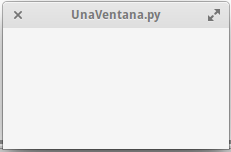
\includegraphics[width=0.5\linewidth]{UnaVentana.png}
	\caption{Ventana creada con el programa de la sección \ref{seccion001} }
	\label{fig1024}
\end{figure}

A continuación explicare cada linea del ejemplo
\begin{lstlisting}[language=Python]
#!/usr/bin/python3
\end{lstlisting}
La primera linea de todos los programas python deben iniciar con \#! seguido por la ruta al interprete Python que se desee utilizar, en nuestro caso es python3.

\begin{lstlisting}[language=Python]
from gi.repository import Gtk
\end{lstlisting}
Para poder acceder a las clases y funciones GTK+ debemos primero importar el módulo Gtk.  La siguiente linea crea una ventana vacía.

\begin{lstlisting}[language=Python]
win = Gtk.Window()
\end{lstlisting}

Seguida por la conexión al evento de la cerrar la ventana para asegurar que la aplicación es terminada cuando se da click en la opción de cerrar ventana.

\begin{lstlisting}[language=Python]
win.connect("delete-event", Gtk.main_quit)
\end{lstlisting}
En el siguiente paso desplegamos la ventana
\begin{lstlisting}[language=Python]
win.show_all()
\end{lstlisting}

Finalmente, generamos un lazo repetido donde se procesa el programa GTK+, el cual se detiene cuando cerramos la ventana

\begin{lstlisting}[language=Python]
GTK.main()
\end{lstlisting}

Para ejecutar el programa, abrimos una terminal, cambiamos al directorio donde se encuentra el archivo, e introducimos:

\begin{lstlisting}[language=bash]
python3 simple_example.py
\end{lstlisting}


\section{Ejemplo 2: Ampliando el Ejemplo}

Un ejemplo clásico y mas útil es la versión PyGObject del programa clásico ``Hola Mundo''.

\begin{lstlisting}[language=Python]
#!/usr/bin/python3
from gi.repository import Gtk

class MiVentana(Gtk.Window):

   def __init__(self):
      Gtk.Window.__init__(self, title="Hola Mundo")
      
      self.boton = Gtk.Button(label="Click Aqui")
      self.boton.connect("clicked", self.on_button_clicked)
      self.add(self.boton)
      
   def on_button_clicked(self, widget):
      print("Hola Mundo")
      
win = MiVentana()
win.connect("delete-event", Gtk.main_quit)
win.show_all()
Gtk.main()
\end{lstlisting}

Este ejemplo es diferente del ejemplo de la sección \ref{seccion001} ya que se utiliza la subclase Gtk.Window para definir nuestra propia clase MiVentana.

\begin{lstlisting}[language=Python]
class MiVentana(Gtk.Window):
\end{lstlisting}

En el constructor de la clase tenemos que llamar al constructor de la super clase. Además, se establece el valor de la propiedad titulo a ``Hola Mundo''.

\begin{lstlisting}[language=Python]
Gtk.Window.__init__(self, title="Hola Mundo")
\end{lstlisting}

Las siguientes tres lineas son utilizadas para crear un widget de boton, conectarlo a la señal clicked y agregarlo al widget de la ventana


\begin{lstlisting}[language=Python]
self.boton = Gtk.Button(label ="Click Aqui")
self.boton.connect("clicked", self.on_button_clicked)
self.add(self.boton)
\end{lstlisting}

Debido a las instrucciones anteriores cuando se de click al boton el método on\_button\_clicked() se ejecutará

\begin{lstlisting}[language=Python]
def on_button_clicked(self, widget):
   print ("Hola Mundo")
\end{lstlisting}

 El último bloque, fuera de la clase, es muy similar al ejemplo simple, pero en lugar de crear una instancia de la clase genérica \textbf{Gtk.Window}, se crea una instancia de \textbf{MiVentana}.

\section{Aspectos importantes del ambiente gráfico GTK+}


Como muchas de las herramientas GUI, GTK+ usa el modelo de programación orientado a eventos. Cuando el usuario no hace nada, GTK+ se sitúa en el lazo principal y espera por una entrada. Si el usuario realiza alguna acción - como dar click con el mouse- entonces el lazo principal ``despierta'' y entrega el evento a GTK+.


Cuando los widget reciben un evento, ellos frecuentemente emiten una o mas señales. Las señales notifican a tu programa que ``Algo interesante ha sucedido'' invocando a las funciones que conectaste a la señal. Tales funciones son llamadas comúnmente \textit{\textbf{callbacks}}. Cuando una \textit{\textbf{callbacks}} es invocada, tu típicamente realizas alguna acción - por ejemplo, cuando se da click sobre un boton de Abrir tu podrías desplegar un dialogo para seleccionar un archivo. Después  de que una rutina \textit{\textbf{callbacks}} termina, GTK+ regresará al lazo principal y esperará por mas entradas del usuario.

Un ejemplo genérico es:

\begin{lstlisting}[language=Python]
handler_id = widget.connect("event", callback, data)
\end{lstlisting}

Primeramente, \textbf{widget} es una instancia de un widget creado anteriormente.En segundo lugar un evento se presenta. Cada widget tiene sus propios y particulares eventos que pueden ocurrir. Por ejemplo, si tienes un botón lo conectarías a un evento clicked. Esto significa que cuando el botón es pulsado, se envía una señal. En tercer lugar, el argumento de la función callback es el nombre de la función callback. Esta función contiene el código que correrá cuando la señal de un tipo específico es enviada. Finalmente, los argumentos de datos incluyen cualquier dato que deba pasarse cuando una señal es enviada. Sin embargo, este argumento es opcional y puede no enviarse sino se requiere.

La función regresa un número que identifica esta particular dupla señal-callback. Se se necesita desconectar la señal de una función callback entonces:


\begin{lstlisting}[language=Python]
widget.disconnect(handler_id)
\end{lstlisting}


Si perdiste el ``handler\_id'' por alguna razón, tu todavia ouedes desconectar la callback específica usando la siguiente funcion

\begin{lstlisting}[language=Python]
widget.disconnect_by_func(callback)
\end{lstlisting}

Casi todas las aplicaciones conectarán la señal del evento ``delete-event'' con la ventana de mas alto nivel. Esta señal es emitida si el usuario requiere que la ventana de mas alto nivel sea cerrada. El manejador por default para esta señal destruye la ventana, pero no termina la aplicación. Conectando la señal ``delete-event'' a la función Gtk.main\_quit resultará en el comportamiento deseado. 


\begin{lstlisting}[language=Python]
window.connect("delete-event", Gtk.main_quit)
\end{lstlisting}

Llamando a la función Gtk.main\_quit() hará que el lazo principal dentro de Gtk.main() termine.

\subsection{Propiedades}

Las propiedades describen el estado y configuración de los widgets. Como con las señales, cada widget tiene su propio conjunto particular de propiedades. Por ejemplo, un boton tiene la propiedad ``label'' la cual contiene el texto de letrero del botón. Tu puedes específicar en nombre y valor de cualquier numero de propiedades como argumentos claves cuando se crea una instancia de un widget. Para crear un texto alineado a la derecha con el texto ``Hola Mundo'' y con un ángulo de 25 grados, usar:

\begin{lstlisting}[language=Python]
label = Gtk.Label(label = "Hola Mundo", angle=25, halign = Gtk.Align.END)
\end{lstlisting}

lo cual es equivalente a:

\begin{lstlisting}[language=Python]
label = Gtk.Label()
label.set_label("Hola Mundo")
label.set_angle(25)
label.set_halign(Gtk.Align.END)
\end{lstlisting}

\section{Cadenas}

En python todas las cadenas son almacenadas como Unicode es una instancia de tipo \textit{\textbf{str}}. Cadenas \textit{\textbf{Encoded}} por otro lado son representados como datos binarios en la forma de instancias de tipo \textbf{\textbf{Byte}}. Conceptualmente, \textit{\textbf{str}} se refiere a texto mientras que \textit{\textbf{bytes}} se refiere a datos. Para convertir de tipo \textit{\textbf{str}} a tipo \textit{\textbf{byte}} se debe usar \textbf{str.encode()} y para convertir de \textit{\textbf{bytes}} a \textit{\textbf{str}} se debe usar \textbf{bytes.decode()}.
Además no es posible mezclar cadenas Unicode con cadenas encoded, porque resulta en un \textbf{TypeError}.

\section{Contenedores de Layout}

Mientras que muchas herramientas de desarrollo GUI te piden la colocación precisa de los widget en una ventana, usando un posicionamiento absoluto, GTK+ utiliza una técnica diferente. En lugar de especificar la posición y tamaño de cada widget en la ventana, tu puedes arreglar tus widgets en columnas, filas y/o tablas. El tamaño de la ventana puede ser determinado automáticamente, basado en los tamaños de los widgets que contiene. Y el tamaño de los widgets son determinados por la cantidad de texto que contiene, o el tamaño mínimo y  máximo que puedes específicar, y/o como requieres que el espacio disponible deba ser compartido entre el conjunto de widgets. Es posible perfeccionar tu layout especificando las distancias y los valores centrales para cada widget. GTK+ entonces utiliza toda esta información para cambiar los posiciones y tamaños cuando el usuario manipula la ventana.

GTK+ arregla los widgets jerarquicamente, usando contenedores. Estos contenedores son invisibles para el usuario final y son insertados en una ventana, o colocados uno dentro de otro de los componentes de layout. Hay dos tipos de contenedores: Contenedores de un solo hijo, de los cuales todos son descendientes de \textbf{Gtk.Bin}, y contenedores de múltiples hijos, de los cuales son descendientes de \textbf{Gtk.Container}. Los contenedores mas usados comúnmente son las cajas verticales u horizontales (\textbf{Gtk.Box}), tablas (\textbf{Gtk.Table}) y redes (\textbf{Gtk.Grid})

\subsection{Cajas}

Las cajas son contenedores invisibles dentro de los cuales podemos empaquetar nuestros widgets. CUando empaquetamos widgets dentro de una caja horizontal, los objetos son colocados horizontalmente de izquierda a derecha dependiendo de donde \textbf{Gtk.Box.pack\_start()} o \textbf{Gtk.Box.pack\_end()} son usados. En una caja vertical, los widgets son empaquetados desde la cima hasta el fondo o vice versa. Es posible usar cualquier combinación de cajas dentro o a lado de otras cajas para crear el efecto deseado.

\subsubsection{Ejemplo de cajas}
\label{seccion003}

Ahora diseñaremos un programa pero con dos botones

\begin{lstlisting}[language=Python]
from gi.repository import Gtk

class MiVentana(Gtk.Window):

   def __init__(self):
      Gtk.Window.__init__(self, title="Hola Mundo")
      self.box = Gtk.Box(spacing = 6)
      self.add(self.box)
      
      self.boton1 = Gtk.Button(label = "Hola")
      self.boton1.connect("clicked", self.on_button1_clicked)
      self.box.pack_start(self.boton1, True, True,0)
      
      self.boton2 = Gtk.Button(label = "Adios")
      self.boton2.connect("clicked", self.on_button2_clicked)
      self.box.pack_start(self.boton2, True, True,0)
      
   def on_button1_clicked(self, widget):
      print("Hola")
   def on_button2_clicked(self, widget):
   print("Adios")

win = MiVentana()
win.connect("delete-event", Gtk.main_quit)
win.show_all()
Gtk.main()

\end{lstlisting}

Primero, se crea una caja orientada horizontalmente en donde los hijos son separados por 6 pixeles. Esta caja es la hija de la ventana principal o de mas alto nivel.

\begin{lstlisting}[language=Python]
self.box = Gtk.Box(spacing = 6)
self.add(self.box)
\end{lstlisting}

Posteriormente, se agregan dos botones en la caja contenedora.

\begin{lstlisting}[language=Python]
self.boton1 = Gtk.Button(label = "Hola")
self.boton1.connect("clicked", self.on_button1_clicked)
self.box.pack_start(self.boton1, True, True,0)
      
self.boton2 = Gtk.Button(label = "Adios")
self.boton2.connect("clicked", self.on_button2_clicked)
self.box.pack_start(self.boton2, True, True,0)

\end{lstlisting}

Mientras que cuando usamos\textbf{ Gtk.Box.pack\_start()} los widgets son posicionados de izquierda a derecha, con  \textbf{Gtk.Box.pack\_end()} son posicionados de derecha a izquierda.

\section{Entrada de datos}

Los widget de entrada permiten al usuario introducir texto. Puedes cambiar el contenido con el método \textbf{Gtk.Entry.set\_text()} y leer el contenido actual con el método \textbf{Gtk.Entry.get\_text()}. Puedes limitar el número de carateres llamando el método \textbf{Gtk.Entry.set\_max\_length()}.

Ocasionalmente querremos hacer una entrada de datos de solo lectura. Esto puede realizarse introduciendo FALSE al método \textbf{Gtk.Entry.set\_editable()}.

Los widgets de entrada de datos pueden también ser usados para pedir password a los usuarios. Es una práctica común ocultar los caracteres que va introduciendo el usuario para prevenir revelar el password a terceros. Llamando al método \textbf{Gtk.Entry.set\_visibility()} con FALSE causa que el texto se oculte.


El widget Gtk.Entry tiene la habilidad de desplegar el progreso o información de la actividad detrás del texto. Esto es similar al widget Gtk.ProgressBar y es comúnmente encontrado en los navegadores web para indicar cuando se ha completado cuando bajas un archivo o página. Para desplegar esta información, usa \textbf{Gtk.Entry.set\_progress\_fraction(}), \textbf{Gtk\_Entry.set\_progress\_pulse\_step(}), o\textbf{ Gtk\_Entry.progress\_pulse()}.

Adicionalmente, cada entrada de texto puede mostrar un ícono a cada lado. Estos íconos se pueden activar pulsando sobre ellos, pueden ser configurados como fuentes de arrastre o tener herramientas enlazadas. Para agregar un ícono, usar \textbf{Gtk.Entry.set\_icon\_from\_stock()} o uno de las otras funciones que le ponen el nombre al ícono, un pixbuf o un tema de ícono. Para ajustar un\textit{ tooltip} a un ícono, usar \textbf{Gtk.Entry.set\_icon\_tooltip\_text()} o la correspondiente función. 

\subsection{Ejemplo}

\begin{lstlisting}[language=Python]
from gi.repository import Gtk, GObject
class EntryWindow(Gtk.Window):
def __init__(self):
Gtk.Window.__init__(self, title="Entry Demo")
self.set_size_request(200, 100)

self.timeout_id = None

vbox = Gtk.Box(orientation=Gtk.Orientation.VERTICAL, spacing=6)
self.add(vbox)

self.entry = Gtk.Entry()
self.entry.set_text("Hello World")
vbox.pack_start(self.entry, True, True, 0)

hbox = Gtk.Box(spacing=6)
vbox.pack_start(hbox, True, True, 0)

self.check_editable = Gtk.CheckButton("Editable")
self.check_editable.connect("toggled", self.on_editable_toggled)
self.check_editable.set_active(True)
hbox.pack_start(self.check_editable, True, True, 0)

self.check_visible = Gtk.CheckButton("Visible")
self.check_visible.connect("toggled", self.on_visible_toggled)
self.check_visible.set_active(True)
hbox.pack_start(self.check_visible, True, True, 0)

self.pulse = Gtk.CheckButton("Pulse")
self.pulse.connect("toggled", self.on_pulse_toggled)
self.pulse.set_active(False)
hbox.pack_start(self.pulse, True, True, 0)

self.icon = Gtk.CheckButton("Icon")
self.icon.connect("toggled", self.on_icon_toggled)
self.icon.set_active(False)
hbox.pack_start(self.icon, True, True, 0)

def on_editable_toggled(self, button):
value = button.get_active()
self.entry.set_editable(value)

def on_visible_toggled(self, button):
value = button.get_active()
self.entry.set_visibility(value)

def on_pulse_toggled(self, button):
if button.get_active():
self.entry.set_progress_pulse_step(0.2)
# Call self.do_pulse every 100 ms
self.timeout_id = GObject.timeout_add(100, self.do_pulse, None)
else:
#Don't call self.do_pulse anymore
GObject.source_remove(self.timeout_id)
self.timeout_id = None
self.entry.set_progress_pulse_step(0)

def do_pulse(self, user_data):
self.entry.progress_pulse()
return True

def on_icon_toggled(self, button):
if button.get_active():
stock_id = Gtk.STOCK_FIND
else:
stock_id = None
self.entry.set_icon_from_stock(Gtk.EntryIconPosition.PRIMARY,
stock_id)

win = EntryWindow()
win.connect("delete-event", Gtk.main_quit)
win.show_all()
Gtk.main()
\end{lstlisting}


\bibliographystyle{acm}
\bibliography{../bibliografia}
\end{document}